\documentclass[12pt, oneside]{uflamon}          % classe base para a monografia

%==============================================================================
% Utilizacao de pacotes
\usepackage[T1]{fontenc}         % usa fontes postscript com acentos
\usepackage[brazil]{babel}       % hifenização e títulos em português do Brasil
\usepackage[utf8]{inputenc}     % permite edição direta com acentos
\usepackage{braket}
\usepackage{amsmath}             % pacote da AMS para Matemática Avançada
\usepackage{amssymb}             % símbolos extras da AMS
\usepackage{latexsym}            % símbolos extras do LaTeX
\usepackage{graphicx}            % para inserção de gráficos
\usepackage{listings}            % para inserção de código
\usepackage{minted}
\usepackage{fancyvrb}            % para inserção de saídas de comandos
%\usepackage{enumerate}           % para personalizar lista enumeradas 
											%(incluso na classe)
\usepackage{longtable}           % para tambelas muito grandes NOVO!!!!

\usepackage{colortbl} % cores em tabelas
\newcolumntype{Z}{|>{\columncolor[gray]{0.9}}l|} %cor cinza em células
%\usepackage{array} % já incluso na classe
\newcolumntype{L}[1]{>{\raggedright\let\newline\\\arraybackslash\hspace{0pt}}m{#1}}
\newcolumntype{C}[1]{>{\centering\let\newline\\\arraybackslash\hspace{0pt}}m{#1}}
\newcolumntype{R}[1]{>{\raggedleft\let\newline\\\arraybackslash\hspace{0pt}}m{#1}}
\usepackage{multirow} % para juntar duas linhas em uma só

\usepackage{multicol} % para uso de várias colunas

% cores para os links cruzados
\usepackage{color}
\definecolor{rltred}{rgb}{0.2,0,0}
\definecolor{rltgreen}{rgb}{0,0.2,0}
\definecolor{rltblue}{rgb}{0,0,0.2}

\usepackage[colorlinks=true,
            urlcolor=rltblue,       % \href{...}{...} external (URL)
            filecolor=rltgreen,     % \href{...} local file
            linkcolor=rltred,       % \ref{...} and \pageref{...}
            citecolor=rltgreen,
            pdftitle={Exemplo de Uso da Classe Uflamon},
          pdfauthor={Joaquim Quinteiro Uchôa},
          pdfsubject={Este texto tem por objetivo servir de exemplo da classe Uflamon.},
          pdfkeywords={Comunicação Científica. 2. Pesquisa . 3. Pesquisa Científica. 
 					 4. Redação. 5. Monografia.}%
]{hyperref} % para referência cruzadas
%\usepackage{hyperref}            % para referência cruzadas
\usepackage{nameref}           % Pacote necessário para \nameref{}
% \usepackage{subfigure}           % figuras dentro de figuras
\usepackage{caption}            % remodelando o formato dos títulos de 
\usepackage{subcaption}           % para subfiguras

\usepackage{tikz}
\usepackage{quantikz}

% configuração padrão do listings   
\lstset{
   language=Java,
   extendedchars=true,
   tabsize=3,
   basicstyle=\footnotesize\ttfamily,
   stringstyle=\em,
   showstringspaces=false 
}

% para referências de acordo com a ABNT
% precisa instalar o abntex2 antes!!!
% http://abntex.codigolivre.org.br/
% comente se pretende usar outro padrão

%abnt-emphasize=bf coloca o título das bibliografias em negrito
%abnt-thesis-year=both
\usepackage[alf,abnt-etal-cite=3,abnt-etal-list=3,abnt-url-package=url,abnt-emphasize=bf]{abntex2cite}

% evite usar o hyperref com abntex, pode dar caca em urls... no linha anterior, informo
% para incluir urls usando o pacote url e não o hyperref
%
% caso queira o hyperref com abntex, comente a linha anterior e descomente a seguinte
%\usepackage[alf,abnt-etal-cite=3,abnt-etal-list=0,abnt-etal-text=emph]{abntex2cite}
%
% caso vc ainda use a versão anterior da abntex, comente a linha incluindo o abntex2cite
% e descomente a próxima linha 
%\usepackage[alf,abnt-etal-cite=3,abnt-etal-list=0,abnt-etal-text=emph]{abntcite}


% redefinindo formatação de títulos de tabelas e figuras


%==============================================================================
% para os fãs do Word, descomente as linhas abaixo
%\sloppy %mais espaço entre as linhas
%\usepackage{identfirst} %identando-se a primeira linha de cada seção
%\noindentfirst % Tire o comentário para manter o padrão do LaTeX.

%==============================================================================
% definido comandos na monografia - não é necessário na sua monografia 
% apenas para exemplificar a definição de novos comandos
\newcommand{\defs}[1]{\textsl{#1}}


% Especificando hifenizações que por ventura LaTeX não saiba fazer
% Por padrão 99,9% dos termos em português devem ser hifenizados corretamente.
\hyphenation{hardware software Li-nux am-bien-te diag-nos-ti-car coor-de-na-ção 
FAE-PE Recovery TelEduc Williams UFLA}

%==============================================================================
% Dados da monografia, capa: autor, titulo, banca, etc... - SUBSTITUA DE ACORDO
%==============================================================================
\author{Marcos Vinicius Figueiredo Sousa}
\title{Métodos de Mitigação e Supressão de ruídos quânticos em QPUs aplicados ao Algoritmo de Grover.}
\engtitle{METHODS FOR MITIGATION AND SUPPRESSION OF QUANTUM NOISE IN QPUS APPLIED TO THE GROVER's ALGORITHM.}
% \subtitle{Exemplo para os Usuários}
% \engtitle{Use of Uflamon Class}
% \engsubtitle{Sample for Users}
% \edicao{3$^a$ edição revista, atualizada e ampliada}
\date{2025}
\tipo{Monografia apresentada à Universidade Federal de Lavras, como parte das exigências do Curso de Engenharia Física, para a obtenção do título de Bacharel.}
% use \orientador ou \orientadora quando for o caso
\orientador{Prof. Dr. Moises Porfírio Rojas Leyva}
%\orientadora{}
% use \coorientador ou \coorientadora quando for o caso
% \coorientadora{Prof. DSc. Maria Orientadora } % comente se não tiver coorientador
%\coorientador{}
\local{Lavras -- MG}
\bancaum{Prof. MSc. Antônio Banca Um}{UFM}
\bancadois{Prof. DSc. João Banca Dois}{FCO} % comente se sua banca tiver só um professor
\bancatres{Profa. Esp. Eliza Banca Três}{BELMIS}
\bancaquatro{Prof. Esp. Carlos Banca Quatro}{IBGPLUS}
\defesa{30 de Fevereiro de 2016}
%==============================================================================
%##################################################
% Dados para Ficha catalográfica, gerada pelo sistema da Biblioteca da UFLA
% http://www.biblioteca.ufla.br/FichaCatalografica/
% dados para ficha catalográfica
% Elaboração da Ficha Catalográfica
\preparofichacat{Ficha catalográfica elaborada pelo Sistema de Geração de Ficha Catalográfica da Biblioteca Universitária da UFLA, com dados informados pelo(a) próprio(a) autor(a).}
% primeiro autor - como na primeira linha da ficha catalográfica
\fcautor{Sousa, Marcos Vinicius Figueiredo}
% autores, separados por vírgula - na ficha catalográfica, no formato que
% vem após o título e a barra ("/")
\fcautores{Marcos Vinicius Figueiredo Sousa}
% caso trabalho seja ilustrado (figuras, gráficos, tabelas, etc.), 
% então informar por meio do comando a seguir
% caso não seja ilustrado, basta comentá-lo
\fcilustrado{il.}
% dados da edição para a ficha 
% \fcedicao{2$^a$ ed. rev., atual. e ampl.}
% tipo do trabalho (tese, dissertação, etc.), de acordo com sistema
% de geração de ficha catalográfica
\fctipo{Monografia (graduação) }
% ano da defesa, só precisa informar se for diferente do ano da publicação
% se forem iguais, comente a linha a seguir
% \fcdatadefesa{2016}
% preencher aqui com os dados de catalogação gerados pelo sistema
\fccatalogacao{1. Ruído Quântico. 2. Interação de qubits. 3. Computação Quântica. I. Leyva, Moises Porfírio Rojas. II. Título.}
% \fcclasi{808.066}

%##################################################

%\antesfichacat{\noindent Para citar este documento: \\UNIVERSIDADE FEDERAL DE LAVRAS. Biblioteca Universitária. \textbf{Manual de normalização e estrutura de trabalhos acadêmicos: TCC, monografias, dissertações e teses}. 2. ed. rev., atual. e ampl. Lavras, 2015. Disponível em: \url{http://www.biblioteca.ufla.br/wordpress/wpcontent/uploads/bdtd/manual_normalizacao_UFLA.pdf}. Acesso em: data de acesso.}

%\depoisfichacat{\noindent A reprodução e a divulgação total ou parcial deste trabalho são autorizadas, por qualquer meio convencional ou eletrônico, para fins de estudo e pesquisa, desde que citada a fonte.\\
%\newline
%{\small Este documento possui páginas em branco para facilitar a impressão frente-e-verso.}}

%##################################################

%##################################################

% para os exemplos do manual
%\newenvironment{exemplomanual}{
%\vspace{0.5cm}
%\noindent\begin{minipage}{\textwidth}
%\noindent\rule{\textwidth}{0.5pt}
%\vspace{-1cm}
%\begin{flushleft}
%}{
%\end{flushleft}
%\vspace{-0.6cm}
%\noindent\rule{\textwidth}{0.5pt}
%\vspace{0.3cm}
%\end{minipage}
%}

%\newenvironment{exemplomanuallista}{
%\vspace{0.3cm}
%\noindent\begin{minipage}{\textwidth - 0.5cm}
%\noindent\rule{\textwidth}{0.5pt}
%\vspace{-1cm}
%\begin{flushleft}
%}{
%\end{flushleft}
%\vspace{-0.6cm}
%\noindent\rule{\textwidth}{0.5pt}
%\vspace{0.3cm}
%\end{minipage}
%}

% por conta de alguns exemplos
%\usepackage{setspace}

%##################################################

% se vc já defendeu e tem o arquivo escaneado da folha de rosto, 
% descomente e altere o nome do arquivo
%\folhaAprovacaoAssinada{folharosto}

% Aqui começa o documento propriamente dito
\begin{document}
\maketitle

\dedic{Espaço reservado a dedicatória.}     % Dedicatórias\\

\thanks{Espaço reservado aos agradecimentos.}         % Agradecimentos

\epigrafe{ % citação opcional
Espaço reservado a epígrafe.\\
(Autor Desconhecido)}

% palavras-chave
\palchaves{Simulação Quântica; Processamento Quântico; Decoerência.}
\resumo{A computação quântica é uma área emergente da ciência da computação que se baseia nos princípios da mecânica quântica para processar informações. Um dos conceitos fundamentais dessa área é a superposição quântica, que permite que os qubits assumam múltiplos estados simultaneamente, possibilitando a realização de cálculos exponencialmente mais rápidos para certos problemas. Um dos algoritmos de destaque nesse contexto, e foco principal deste trabalho, é o Algoritmo de Grover, utilizado para busca em bases de dados não estruturadas, proporcionando uma aceleração quadrática em relação aos métodos clássicos. Este estudo tem como objetivo analisar a estrutura e o funcionamento do Algoritmo de Grover, avaliando sua eficiência teórica e prática por meio de cálculos analíticos, simulações computacionais e implementações em hardwares quânticos reais. Além disso, serão exploradas técnicas para aprimorar a confiabilidade das execuções em dispositivos quânticos físicos, que são susceptíveis a erros devido à presença de ruído quântico, originado principalmente da interação entre os qubits e o ambiente. Para transpor esses desafios, serão investigados métodos de otimização, supressão e mitigação de ruído, buscando melhorar a precisão dos resultados obtidos nas \textit{Quantum Processing Units} (QPUs). Dessa forma, este trabalho pretende não apenas aprofundar o conhecimento sobre a implementação e aplicabilidade do Algoritmo de Grover, mas também avaliar estratégias que aumentem sua robustez em ambientes ruidosos, contribuindo para o avanço da computação quântica.}  % Resumo (digite aqui o resumo)

% keywords devem vir antes do abstract
\keywords{Quantum Simulation; Quantum Processing; Decoherence.} % keywords
\abstract{Quantum computing is an emerging field of computer science that is based on the principles of quantum mechanics to process information. One of its fundamental concepts is quantum superposition, which allows qubits to exist in multiple states simultaneously, enabling exponentially faster computations for certain problems. One of the prominent algorithms in this context, and the main focus of this work, is Grover's Algorithm, which is used for searching in unstructured databases, providing a quadratic speedup compared to classical methods. This study aims to analyze the structure and functioning of Grover's Algorithm, evaluating its theoretical and practical efficiency through analytical calculations, computational simulations, and implementations on real quantum hardware. In addition, techniques will be explored to enhance the reliability of executions on physical quantum devices, which are susceptible to errors due to the presence of quantum noise, primarily caused by the interaction between qubits and the environment. To overcome these challenges, methods of noise optimization, suppression, and mitigation will be investigated, seeking to improve the accuracy of results obtained in Quantum Processing Units (QPUs). Thus, this work aims not only to deepen the understanding of the implementation and applicability of Grover's Algorithm but also to evaluate strategies that increase its robustness in noisy environments, contributing to the advancement of quantum computing}

%##################################################

\impacto{O presente trabalho promove impactos significativos nos campos tecnológico e educacional, além de contribuir potencialmente para avanços econômicos e sociais a longo prazo. Do ponto de vista tecnológico, a pesquisa auxilia no desenvolvimento de técnicas que aumentam a confiabilidade e, por conseguinte, a aplicabilidade dos computadores quânticos, permitindo uma maior fidelidade nos resultados obtidos e reduzindo as limitações impostas pelos ruídos quânticos intrínsecos às atuais \textit{Quantum Processing Units} (QPUs). Esses avanços são fundamentais para acelerar a adoção da computação quântica em setores estratégicos, como criptografia, inteligência artificial e otimização de processos industriais. No âmbito acadêmico e educacional, o estudo pode agir como um fomentador da formação de novos pesquisadores e profissionais capacitados, ao instigar o desenvolvimento de novas áreas de pesquisa e ainda integrar conhecimentos teóricos e experimentais essenciais para o avanço da computação quântica no Brasil. A pesquisa contribui diretamente para a área temática de Tecnologia e Produção da Política Nacional de Extensão, uma vez que busca aprimorar a aplicabilidade de algoritmos quânticos e desenvolver técnicas de mitigação de erros aplicáveis a diferentes domínios. Além disso, o projeto está alinhado com os Objetivos de Desenvolvimento Sustentável (ODS) da ONU, especialmente o ODS 9, que incentiva a inovação o fortalecimento de pesquisas científicas em países em desenvolvimento, como é o caso do Brasil, e o ODS 4, que visa a educação de qualidade, pois o estudo promove o ensino e a pesquisa em computação quântica no país, uma vez que é apresentado de forma didática e de fácil entendimento. Embora os impactos diretos ainda sejam mais perceptíveis no ambiente acadêmico e de pesquisa, o desenvolvimento de técnicas de mitigação de ruído tem o potencial de beneficiar indústrias e empresas que futuramente empregarão a computação quântica para resolver problemas complexos em menor tempo e com maior eficiência. Dessa forma, este trabalho representa um passo relevante para a evolução da computação quântica e sua aplicabilidade prática, fortalecendo o Brasil como um agente ativo nessa revolução tecnológica global.}

\impact{This work promotes significant impacts in the technological and educational fields, as well as potentially contributing to long-term economic and social advances. From a technological perspective, the research aids in the development of techniques that enhance the reliability and, consequently, the applicability of quantum computers, enabling greater fidelity in the results obtained and reducing the limitations imposed by the intrinsic quantum noise present in current Quantum Processing Units (QPUs). These advances are essential for accelerating the adoption of quantum computing in strategic sectors such as cryptography, artificial intelligence, and industrial process optimization. In the academic and educational sphere, the study can act as a catalyst for the training of new researchers and skilled professionals by encouraging the development of new research areas while integrating theoretical and experimental knowledge essential for the advancement of quantum computing in Brazil. The research directly contributes to the Technology and Production area of the National Extension Policy, as it seeks to improve the applicability of quantum algorithms and develop error mitigation techniques applicable to different domains. Furthermore, the project aligns with the United Nations Sustainable Development Goals (SDGs), particularly SDG 9, which promotes innovation and strengthens scientific research in developing countries, such as Brazil, and SDG 4, which aims for quality education, as the study fosters teaching and research in quantum computing in the country, presenting the topic in a didactic and easily understandable manner. Although the direct impacts are still more noticeable in the academic and research environment, the development of noise mitigation techniques has the potential to benefit industries and companies that will eventually employ quantum computing to solve complex problems in less time and with greater efficiency. Thus, this work represents a significant step toward the evolution of quantum computing and its practical applicability, strengthening Brazil as an active player in this global technological revolution.}
%##################################################

% Dados do guia
%\begin{titlepage}
%\pagestyle{empty}
%\renewcommand{\baselinestretch}{1}
%\enlargethispage{1.5cm}
%\input{reitoria}
%\cleardoublepage
%\end{titlepage}

%##################################################

% descomente para habilitar a lista desejada
\listoffigures                             % Lista de Figuras
%\listofilustracoes
\listofgraficos						       % Lista de Gráficos
% \listoftables                            % Lista de Tabelas
% \listofquadros							   % Lista de Quadros
%\listofexemplos
%\listofteoremas
\listofsimbolos
\tableofcontents                           % Sumário

\clearpage

\pagestyle{ufla}

%==============================================================================
% incluindo os capitulos
\setcounter{page}{1} % Reinicia a numeração da página
\chapter{INTRODUÇ\~{A}O}
\label{chap:introducao}

No início do desenvolvimento dos primeiros computadores, com a \emph{M\'{a}quina de Turing} em 1936 e, posteriormente, a criaç\~{a}o dos transistores nos Laboratórios da \emph{Bell Telephone}, em 1947 \cite{transistor_hist}, e sua evoluç\~{a}o at\'{e} passar a ser utilizado na construç\~{a}o de processadores, muito j\'{a} se pensava a respeito dos incríveis feitos que essa emergente tecnologia poderia proporcionar, e realmente podemos ver tal expectativa sendo concretizada nos dias atuais, com os computadores sendo acessíveis at\'{e} mesmo da palma da m\~{a}o, com os \textit{smartphones}, algo inimagin\'{a}vel àquela \'{e}poca.

Contudo, embora ainda seja – e continuar\~{a}o sendo – demasiadamente útil, existem novos problemas que exigem uma forma diferente de processamento, como Richard Feynman afirmou em 1981 na primeira Confer\^{e}ncia da Física da Computaç\~{a}o, na qual sugeriu que computadores qu\^{a}nticos poderiam realizar simulações que s\~{a}o impossíveis de serem realizadas pelos computadores cl\'{a}ssicos, mesmo aqueles mais robustos. Isso se deve à natureza intrínseca aos próprios problemas, como, por exemplo, a simulaç\~{a}o de mol\'{e}culas grandes ou materiais complexos, que exigem um poder de processamento que cresce exponencialmente com o aumento do número de partículas. Em adiç\~{a}o, Feynman tamb\'{e}m descreveu o mundo físico como “qu\^{a}ntico”, e como tal, sistemas físicos (qu\^{a}nticos) apenas seriam adequadamente simulados por meio de computadores que utilizassem princípios qu\^{a}nticos de processamento \cite{feynman1982}.

A partir desse ponto, muitos adeptos e fomentadores da ideia contribuíram com conhecimento, como David Deutsch, que propôs o primeiro algoritmo qu\^{a}ntico, mesmo que com aplicações limitadas, foi demonstrada uma efici\^{e}ncia muito superior aos algoritmos cl\'{a}ssicos \cite{deutsch1985}, al\'{e}m de servir de suporte para o desenvolvimento de outros algoritmos importantes, como os Algoritmos de Simon \cite{simon1994} e de Shor . Tamb\'{e}m Peter Shor mostrou com seu algoritmo qu\^{a}ntico de fatoraç\~{a}o que um algoritmo qu\^{a}ntico poderia fatorar números inteiros exponencialmente mais r\'{a}pido que algoritmos cl\'{a}ssicos \cite{shor1994}. E, ainda, Lov Grover, que apresentou um algoritmo de busca em listas desordenadas, que opera por meio de uma t\'{e}cnica de amplificaç\~{a}o tanto de amplitudes quanto das probabilidades e que possui melhora quadr\'{a}tica na efici\^{e}ncia em relaç\~{a}o a m\'{e}todos cl\'{a}ssicos conhecidos \cite{grover1996}. 

Seguindo o vi\'{e}s j\'{a} apresentado, este trabalho tem por objetivo se envolver no estudo, construç\~{a}o, melhoria de resultados e an\'{a}lise do Algoritmo de Grover aplicado a um sistema de quatro qubits, a fim de melhor compreend\^{e}-lo, e ainda conseguir gerar conteúdo que poder\'{a} ser base para novos trabalhos. As melhorias propostas neste trabalho est\~{a}o relacionadas aos m\'{e}todos de supress\~{a}o – que \'{e} uma estrat\'{e}gia preventiva, aplicada durante a execuç\~{a}o do circuito qu\^{a}ntico para minimizar a geraç\~{a}o de erros – e de mitigaç\~{a}o – ocorre após a execuç\~{a}o do circuito qu\^{a}ntico, com t\'{e}cnicas que tentam corrigir ou compensar os erros nos resultados obtidos – de ruídos qu\^{a}nticos gerados pelas \textit{Quantum Processing Unit} (QPUs) nos Computadores Qu\^{a}nticos (CQs). Ambas estrat\'{e}gias possuem diversos m\'{e}todos incluídos no \emph{Qiskit}, alguns deles ser\~{a}o empregados, suas influ\^{e}ncias na qualidade final dos resultados ser\~{a}o analisadas e discutidas no discorrer deste texto.

\chapter{FUNDAMENTAÇ\~{a}O TEÓRICA}
\label{chap:fundamentacao}

A computaç\~{a}o qu\^{a}ntica vem ganhando destaque por sua capacidade de solucionar problemas considerados intrat\'{a}veis para sistemas cl\'{a}ssicos. Entre os algoritmos qu\^{a}nticos, o Algoritmo de Grover se destaca por oferecer uma melhoria quadr\'{a}tica na busca em bases de dados n\~{a}o estruturadas. Entretanto, a presença de ruídos nas QPUs – oriundos de fontes como decoer\^{e}ncia, interaç\~{a}o com o meio, imperfeições nas operações qu\^{a}nticas, dentre outras – impõe desafios que requerem a implementaç\~{a}o de estrat\'{e}gias que tornem os erros menos impactantes no resultado final. Este referencial teórico visa fundamentar os conceitos necess\'{a}rios para a compreens\~{a}o tanto do funcionamento e posterior implementaç\~{a}o do Algoritmo de Grover quanto dos m\'{e}todos de supress\~{a}o e mitigaç\~{a}o de ruídos que ser\~{a}o aplicados.

Na computaç\~{a}o qu\^{a}ntica, os \textit{quantum bits}, ou bits qu\^{a}nticos – chamados de \textit{qubits} – s\~{a}o a unidade fundamental de informaç\~{a}o. Diferente dos bits cl\'{a}ssicos, que assumem apenas os valores $0$ ou $1$, os qubits podem assumir estados de superposiç\~{a}o, que podemos entender como uma condiç\~{a}o em que o qubit “pode tamb\'{e}m assumir os dois valores simultaneamente. Nessa situaç\~{a}o, diz-se que  um  qubit  est\'{a}  em  superposiç\~{a}o  de  estados,  ou  coer\^{e}ncia” \cite{Cuzziol2023_Superposicao}; al\'{e}m disso, o computador qu\^{a}ntico \'{e} capaz de realizar o processamento paralelo das informações contidas nos qubits, denominado de paralelismo qu\^{a}ntico – quer dizer, o CQ consegue atuar em todos os qubits de forma síncrona, logo, \'{e} possível processar toda a informaç\~{a}o simultaneamente. Um outro conceito extremamente importante quando se fala n\~{a}o apenas de computaç\~{a}o qu\^{a}ntica especificamente, mas presente no cerne da mec\^{a}nica qu\^{a}ntica, \'{e} o que chamamos de emaranhamento qu\^{a}ntico, que \'{e} uma “consequ\^{e}ncia direta da condiç\~{a}o de superposiç\~{a}o” \cite{Rigolin2008_Emaranhamento}, e, em palavras simples, pode ser entendido como uma forte correlaç\~{a}o entre diferentes partículas, de modo que o estado de uma n\~{a}o pode ser descrito de forma desvinculada ao estado da outra, independentemente da dist\^{a}ncia que as separam, devido ao princípio da n\~{a}o localidade, que Einstein chama de “aç\~{a}o fantasmagórica à dist\^{a}ncia”. Ainda segundo Rigolin \citeyear{Rigolin2008_Emaranhamento}, “os estados emaranhados podem ainda serem usados para se realizar eficientemente tarefas impossíveis de serem executadas por meio de recursos cl\'{a}ssicos [...], como o teletransporte qu\^{a}ntico”.

Os \textit{chips} qu\^{a}nticos da IBM (QPUs) operam utilizando qubits supercondutores, que s\~{a}o projetados para reduzir a sensibilidade ao ruído de carga e aumentar a estabilidade dos estados qu\^{a}nticos. Para manter a supercondutividade, esses qubits operam a temperaturas extremamente baixas, próximas do zero absoluto. Esses qubits s\~{a}o manipulados pelas portas lógicas qu\^{a}nticas, isto \'{e}, o estado de qubit \'{e} modificado pela aplicaç\~{a}o de pulsos eletromagn\'{e}ticos de micro-ondas que induzem transições nos níveis de energia dos mesmos \cite{EITCA2024_CQ}
Dentre as portas lógicas qu\^{a}nticas existentes, podem ser citadas algumas como, por exemplo, as portas \emph{Hadamard} (\simboloinline{$H$}{Porta Lógica Quântica Hadamard}), \emph{Pauli-X} (\simboloinline{$X$}{Porta Lógica Quântica $X$}), \emph{Pauli-Z} (\simboloinline{$Z$}{Porta Lógica Quântica $Z$}), \emph{X-Controlada} (\simboloinline{$C_x,~CNOT$}{Porta Lógica Quântica $C_X$ ou $CNOT$}), \emph{Z-Controlada} (\simboloinline{$C_Z$}{Porta Lógica Quântica $C_Z$}) e a porta  \emph{Toffoli} (\emph{X-Multi-Controlada} de tr\^{e}s qubits (\simboloinline{$MCX$}{Porta Lógica Quântica $MCX$}), que s\~{a}o portas lógicas qu\^{a}nticas muito conhecidas, e disponíveis no \emph{Qiskit}, e quase todas ser\~{a}o abordadas no decorrer deste documento, visto que ser\~{a}o necess\'{a}rias para a construç\~{a}o do circuito qu\^{a}ntico (mais detalhes sobre construç\~{a}o e operaç\~{a}o de cada uma ser\~{a}o dados no Cap\'{i}tulo~\ref{chap:procedimentos}). Essas portas lógicas operam de forma a explorar as peculiaridades da mec\^{a}nica qu\^{a}ntica para efetuar c\'{a}lculos complexos \cite{Nielsen_Chuang2010_Livro}.

O Algoritmo de Grover, foco deste objeto, foi proposto por Grover \citeyear{grover1996} e tem como objetivo acelerar a busca em bases de dados n\~{a}o ordenadas. Seu funcionamento pode ser resumido em tr\^{e}s etapas principais: inicializaç\~{a}o, em que h\'{a} a criaç\~{a}o do Espaço de Pesquisa, que nada mais \'{e} que a superposiç\~{a}o uniforme de todos os estados possíveis; aplicaç\~{a}o do or\'{a}culo, uma operaç\~{a}o que marca (adicionando uma fase negativa) o(s) estado(s) que correspondem à soluç\~{a}o do problema; e, por fim, aplicaç\~{a}o do Operador de Difus\~{a}o ou de Amplificaç\~{a}o, que amplifica a probabilidade do estado marcado, tornando-o mais prov\'{a}vel de ser medido \cite{qiskit_GroverNotebook}. A efici\^{e}ncia do algoritmo de Grover se evidencia na sua capacidade de reduzir o número de buscas necess\'{a}rias em comparaç\~{a}o com os m\'{e}todos cl\'{a}ssicos, o que o torna uma ferramenta promissora em diversas aplicações, como a quebra de sistemas criptogr\'{a}ficos e otimizaç\~{a}o de buscas \cite{grover1996}.

Apesar do potencial dos algoritmos qu\^{a}nticos, os computadores qu\^{a}nticos atuais sofrem com a presença de ruído – decorrente de decoer\^{e}ncia dos qubits, imperfeições nas portas lógicas, interaç\~{a}o com o meio e erros de leitura. Esses fatores podem degradar significativamente a fidelidade dos resultados dos algoritmos, e uma fidelidade alta \'{e} crucial para garantir que os estados qu\^{a}nticos sejam preservados com alta precis\~{a}o durante as operações \cite{jozsa1994_Fidelidade}. Tomando por base esta asserç\~{a}o, fica evidente a necessidade e a import\^{a}ncia da utilizaç\~{a}o de m\'{e}todos que possam restringir a influ\^{e}ncia do ruído qu\^{a}ntico, de modo a garantir fidelidades maiores nos estados finais após as operações, gerando, por conseguinte, melhores e mais confi\'{a}veis resultados. 

O \emph{Qiskit SDK} possui uma gama de ferramentas para supress\~{a}o e mitigaç\~{a}o de ruído qu\^{a}ntico, e \'{e} intuito deste trabalho aplicar algumas delas ao circuito qu\^{a}ntico e analisar suas efetividades, emph{i. e.}, a capacidade de cada m\'{e}todo de melhorar o resultado final. S\~{a}o eles: Otimizaç\~{a}o do circuito compilado, Desacoplamento Din\^{a}mico (\simboloinline{DD}{\textit{Dynamical Decoupling}}), Compilaç\~{a}o Aleatória (\textit{Pauli Twirling}),  Extrapolaç\~{a}o de Erro Zero (\simboloinline{ZNE}{\textit{Zero-Noise Extrapolation}}), Extinç\~{a}o de Erro de Leitura Giratória (\simboloinline{TREX}{\textit{Twirled Readout Error eXtinction}}), Amplificaç\~{a}o de Erro Probabilístico (\simboloinline{PEA}{\textit{Probabilistic Error Amplification}}), Cancelamento de Erro Probabilístico (\simboloinline{PEC}{\textit{Probabilistic Error Cancellation}}).

\section{M\'{e}todos de Supress\~{a}o e Mitigaç\~{a}o}
\label{sec: supressaoMitigacao}

Como discutido por Preskill \citeyear{Preskill2018_NISQ}, o mundo experimenta no cen\'{a}rio atual a era da tecnologia Qu\^{a}ntica de Escala Intermedi\'{a}ria Ruidosa (\simboloinline{NISQ}{\textit{Noisy Intermediate-Scale Quantum}}, na sigla em ingl\^{e}s para \textit{Noisy Intermediate-Scale Quantum}), que descreve o “tamanho” dos CQs dispon\'{i}veis atualmente em termos de quantidade de qubits (entre $50$ e algumas centenas), enquanto o termo “ruidoso” faz jus ao objeto de estudo desta produç\~{a}o: ru\'{i}do qu\^{a}ntico, que, ainda segundo ele, adv\'{e}m da incapacidade de se controlar fielmente as interaç\~{o}es dos qubits. 

\begin{quote}
    “[...] com esses dispositivos barulhentos n\~{a}o esperamos ser capazes de executar um circuito que contenha muito mais do que cerca de 1000 portas — isto \'{e}, 1000 operaç\~{o}es fundamentais de dois qubits — porque o ru\'{i}do sobrecarregar\'{a} o sinal em um circuito muito maior do que isso. Essa limitaç\~{a}o no tamanho do circuito imp\~{o}e um teto ao poder computacional da tecnologia NISQ. Eventualmente, faremos melhor, usando correç\~{a}o de erro qu\^{a}ntico para escalar para circuitos maiores.” \cite{Preskill2018_NISQ}.
\end{quote}

Dado o exposto, torna-se imprescind\'{i}vel a utilizaç\~{a}o de pelo menos alguns dos m\'{e}todos que ser\~{a}o aqui introduzidos, cabendo ao usu\'{a}rio optar por aqueles que mais se adequam às caracter\'{i}sticas intr\'{i}nsecas a cada circuito, espec\'{i}ficas de cada aplicaç\~{a}o. \'{e} esperado que este comp\^{e}ndio seja \'{u}til para servir de fonte de pesquisa para auxiliar nessa tomada de decis\~{a}o.

\subsection{Supress\~{a}o}
\label{subSec: supressao}


As t\'{e}cnicas de supress\~{a}o de ru\'{i}do em computaç\~{a}o qu\^{a}ntica visam reduzir o surgimento do ru\'{i}do durante o processamento ou execuç\~{a}o do circuito (como decoer\^{e}ncia e erros de porta), e, por conseguinte, evitar os efeitos indesejados sem recorrer, necessariamente, a códigos completos de correç\~{a}o de erros. Essas t\'{e}cnicas s\~{a}o especialmente relevantes no contexto dos dispositivos NISQ, onde a presença de ru\'{i}do ainda \'{e} significativa. As t\'{e}cnicas de supress\~{a}o contempladas pelo \emph{Qiskit} e que aqui tamb\'{e}m o ser\~{a}o, s\~{a}o:

\subsubsection*{Otimizaç\~{a}o do Circuito Qu\^{a}ntico}
\label{subSubSec: otimizacao}

A otimizaç\~{a}o ocorre na fase de compilaç\~{a}o, e \'{e} um m\'{e}todo que deve ser utilizado durante o processo de mapeamento do circuito qu\^{a}ntico virtual\footnote{Um circuito qu\^{a}ntico virtual refere-se à representaç\~{a}o abstrata e idealizada de um circuito qu\^{a}ntico, em que n\~{a}o h\'{a} interfer\^{e}ncia de ru\'{i}dos qu\^{a}nticos ou limitaç\~{o}es tecnológicas da implementaç\~{a}o f\'{i}sica.} para o circuito qu\^{a}ntico f\'{i}sico\footnote{
Um circuito qu\^{a}ntico f\'{i}sico \'{e} aquele implementado em hardware real, tamb\'{e}m chamado \textit{backend}, utilizando as portas lógicas que o mesmo suporta.
} utilizando para isso a funç\~{a}o “transpile”, que possui quatro poss\'{i}veis n\'{i}veis: n\'{i}vel $0$, que n\~{a}o h\'{a} otimizaç\~{a}o; n\'{i}vel $1$, que combina decomposiç\~{a}o otimizada de portas de um qubit com cancelamento de portas inversas consecutivas; n\'{i}vel $2$, que utiliza um m\'{e}todo de cancelamento comutativo em vez de cancelamento de $C_X$'s, resultando na diminuiç\~{a}o de portas redundantes; n\'{i}vel $3$, que \'{e} o n\'{i}vel de otimizaç\~{a}o mais eficaz, embora mais exigente em se tratando de poder computacional, pois emprega v\'{a}rios m\'{e}todos, inclusive decomposiç\~{a}o otimizada de portas de um qubit, usada no n\'{i}vel um, e cancelamento comutativo aplicado no n\'{i}vel dois, al\'{e}m de outros m\'{e}todos como coleç\~{a}o de subcircuitos de dois qubits, consolidaç\~{a}o de portas lógicas (blocos) consecutivas atuantes em um mesmo qubit para um \'{u}nico bloco mais otimizado, e, por fim, utiliza s\'{i}ntese unit\'{a}ria, que pode fazer uma simplificaç\~{a}o das portas por suas portas-base \cite{IBM2025_transpile}.

\textbf{Decomposiç\~{a}o Otimizada de Portas de um Qubit} \cite{IBM2025_OptimGates1qb}: Esse m\'{e}todo visa otimizar cadeias de portas de qubit \'{u}nico combinando-as em uma \'{u}nica porta. As condiç\~{o}es empregadas pelo algoritmo para tomar a decis\~{a}o de substituir o conjunto original de portas por uma nova configuraç\~{a}o s\~{a}o:
se a corrente original estava fora da base: substituir;
se a cadeia original estava na base, mas a ress\'{i}ntese \'{e} menor erro: substituir;
se a cadeia original cont\'{e}m uma porta de pulso: n\~{a}o substitua;
se a cadeia original equivale à identidade: substituir por nulo;
O erro \'{e} calculado como uma multiplicaç\~{a}o dos erros de portas individuais naquele qubit.

\textbf{Cancelamento Inverso} \cite{IBM2025_CancelInverso}: O objetivo desse m\'{e}todo \'{e} identificar e remover pares de portas qu\^{a}nticas consecutivas que s\~{a}o inversas uma da outra, otimizando assim o circuito ao eliminar operaç\~{o}es redundantes. Ao aplic\'{a}-lo, \'{e} poss\'{i}vel reduzir a profundidade do circuito e minimizar poss\'{i}veis fontes de erro, contribuindo para a execuç\~{a}o mais eficiente de algoritmos qu\^{a}nticos.

\textbf{Cancelamento Comutativo }\cite{IBM2025_CancelComutativo}: O objetivo desse m\'{e}todo \'{e} identificar e remover portas auto-inversas redundantes, aproveitando as relaç\~{o}es de comutaç\~{a}o no circuito. As portas consideradas incluem: $H$, $X$, $Y$, $Z$, $C_X$, $C_Y$, $C_Z$. Ao aplic\'{a}-lo, \'{e} poss\'{i}vel reduzir a complexidade do circuito, eliminando operaç\~{o}es redundantes e melhorando a efici\^{e}ncia da execuç\~{a}o em dispositivos qu\^{a}nticos.

\textbf{Coleç\~{a}o de Subcircuitos de 2 Qubits} \cite{IBM2025_ColetaBlock2qb}: \'{e} uma ferramenta de an\'{a}lise que identifica e agrupa subcircuitos compostos por portas de dois qubits que s\~{a}o adjacentes (vizinhas) e atuam nos mesmos qubits. Esses blocos coletados podem ser posteriormente otimizados ou sintetizados de maneira mais eficiente por outras passagens do \textit{transpile}. Ao utiliz\'{a}-la, \'{e} poss\'{i}vel preparar o circuito para otimizaç\~{o}es subsequentes, como a consolidaç\~{a}o de operaç\~{o}es ou a reduç\~{a}o da profundidade do circuito, melhorando a efici\^{e}ncia da execuç\~{a}o em dispositivos qu\^{a}nticos.

\textbf{Consolidaç\~{a}o de Blocos de Portas Consecutivas} \cite{IBM2025_ConsolidaBlocos}: Essa \'{e} uma transformaç\~{a}o que substitui sequ\^{e}ncias de portas consecutivas atuando nos mesmos qubits por um \'{u}nico nó unit\'{a}rio. Geralmente, esses blocos s\~{a}o selecionados anteriormente por outra ferramenta, como a Coleç\~{a}o de Subcircuitos de 2 Qubits. Essa consolidaç\~{a}o permite que o subcircuito seja ressincronizado posteriormente, potencialmente resultando em uma implementaç\~{a}o mais otimizada. Al\'{e}m disso, \'{e} poss\'{i}vel reduzir a complexidade do circuito, agrupando operaç\~{o}es em unidades \'{u}nicas que podem ser mais eficientes para execuç\~{a}o em hardware qu\^{a}ntico.

\textbf{S\'{i}ntese Unit\'{a}ria} \cite{IBM2025_SinteseUnit}: O objetivo dessa funç\~{a}o \'{e} sintetizar operaç\~{o}es unit\'{a}rias, substituindo sequ\^{e}ncias de portas por implementaç\~{o}es equivalentes que sejam mais eficientes ou que atendam a restriç\~{o}es espec\'{i}ficas do hardware. Funciona atrav\'{e}s da an\'{a}lise do circuito em busca de subcircuitos unit\'{a}rios e os reescreve utilizando um conjunto espec\'{i}fico de portas base, visando otimizar o circuito de acordo com as caracter\'{i}sticas do \textit{backend} (CQ) alvo.

\subsubsection*{Desacoplamento Din\^{a}mico (DD, \textit{Dynamical Decoupling})}
\label{subSubSec: DD}

“Circuitos qu\^{a}nticos s\~{a}o executados em hardware IBM como sequ\^{e}ncias de pulsos de micro-ondas que precisam ser agendados e executados em intervalos de tempo precisos.” \cite{IBM_DD}. Durante uma operaç\~{a}o qualquer, alguns qubits podem passar alguns intervalos de tempo sem que estejam sendo utilizados, devido à exist\^{e}ncia de lacunas nos circuitos; esses qubits podem acabar interagindo entre si de forma n\~{a}o controlada e indevida. Essas interaç\~{o}es s\~{a}o respons\'{a}veis por gerar quantidades significativas de erros no resultado final. O DD \'{e} muito \'{u}til para este tipo de circuitos, onde h\'{a} lacunas, pois “\'{e} uma t\'{e}cnica de controle qu\^{a}ntico que consiste em aplicar sequ\^{e}ncias personalizadas de pulsos ao sistema qu\^{a}ntico considerado para cancelar (ou fazer a m\'{e}dia) da interaç\~{a}o com o ambiente” \cite{lopez2023_DD}, ou seja, s\~{a}o inseridas sequ\^{e}ncias de pulsos de micro-ondas nos qubits ociosos que s\~{a}o propositalmente sim\'{e}tricos, para que sua m\'{e}dia total seja cancelada, de modo que se equivalham à operaç\~{a}o de identidade, isto \'{e}, n\~{a}o causem perturbaç\~{o}es no sistema. Esses pulsos controlados agem de modo a suprimir erros de interaç\~{a}o indevida, ao impedir que haja a interaç\~{a}o entre qubits. 

\subsubsection*{Compilaç\~{a}o Aleatória (\textit{Randomized Compiling} ou \textit{Pauli Twirling})}
\label{subSubSec: twirling}

O m\'{e}todo de \textit{Pauli twirling} \'{e} uma t\'{e}cnica de supress\~{a}o de erros que transforma canais de ru\'{i}do arbitr\'{a}rios em canais do tipo Pauli, os quais s\~{a}o mais f\'{a}ceis de modelar e corrigir. A ideia central \'{e} aplicar, de forma aleatória, operaç\~{o}es do grupo de Pauli – como os operadores $I$, $X$, $Y$ e $Z$ – antes e depois de um canal de ru\'{i}do. Ao se fazer a m\'{e}dia (ou "\textit{twirling}") sobre essa distribuiç\~{a}o aleatória de operaç\~{o}es, os termos n\~{a}o diagonais (ou seja, os erros coerentes) tendem a se cancelar, resultando em um canal de ru\'{i}do que age de forma puramente estoc\'{a}stica\footnote{Um erro estoc\'{a}stico ocorre de forma aleatória, seguindo uma distribuiç\~{a}o probabil\'{i}stica, ao contr\'{a}rio dos erros coerentes, que se manifestam de maneira sistem\'{a}tica. Esse comportamento possibilita que t\'{e}cnicas de correç\~{a}o e mitigaç\~{a}o sejam aplicadas de forma mais eficaz, pois os efeitos do ru\'{i}do podem ser tratados estatisticamente \cite{Nielsen_Chuang2010_Livro}}.
Em outras palavras, o ru\'{i}do original, que pode apresentar comportamentos complexos e coerentes, \'{e} transformado em um ru\'{i}do que se comporta como uma mistura probabil\'{i}stica de erros simples (por exemplo, erros de \textit{bit-flip} ou \textit{phase-flip}). Essa transformaç\~{a}o facilita tanto a an\'{a}lise teórica quanto a mitigaç\~{a}o pr\'{a}tica dos erros, pois canais de ru\'{i}do do tipo Pauli s\~{a}o bem compreendidos e possuem uma estrutura que pode ser incorporada em protocolos de correç\~{a}o de erros e t\'{e}cnicas de mitigaç\~{a}o, como o \textit{randomized benchmarking}.
\begin{quote}
    
"Realizado sozinho, ele pode mitigar ru\'{i}do coerente porque o ru\'{i}do coerente tende a se acumular quadraticamente com o n\'{u}mero de operaç\~{o}es, enquanto o ru\'{i}do de Pauli se acumula linearmente. O twirling de Pauli \'{e} frequentemente combinado com outras t\'{e}cnicas de mitigaç\~{a}o de erros que funcionam melhor com ru\'{i}do de Pauli do que com ru\'{i}do arbitr\'{a}rio" \cite{IBM_PauliTwirling}.
\end{quote}
Conforme discutido por Emerson et al. \citeyear{emerson2005_PauliTwirling}, essa t\'{e}cnica \'{e} fundamental para converter erros que se acumulam de maneira prejudicial em erros estoc\'{a}sticos, cuja influ\^{e}ncia pode ser controlada e, em muitos casos, mitigada atrav\'{e}s de m\'{e}todos de pós-processamento. Trabalhos posteriores, como o de Temme et al.  \citeyear{temme2017_PauliTwirling}, demonstram aplicaç\~{o}es pr\'{a}ticas dessa t\'{e}cnica para melhorar a fidelidade de circuitos qu\^{a}nticos de curta profundidade, tornando os resultados experimentais mais próximos do ideal.

\subsection{Mitigaç\~{a}o}
\label{subSec: mitigacao}

T\'{e}cnicas de mitigaç\~{a}o s\~{a}o utilizadas como complemento às de supress\~{a}o, aplicadas no pós-processamento com o intuito de compensar os efeitos dos erros induzidos nos resultados medidos pela aç\~{a}o do ru\'{i}do que n\~{a}o pôde ser totalmente cancelado na supress\~{a}o.

\subsubsection*{Extinç\~{a}o de Erro de Leitura Giratória (TREX, \textit{Twirled Readout Error eXtinction})}
\label{subSubSec: trex}

O \textit{Twirled Readout Error eXtinction} (TREX) \'{e} uma t\'{e}cnica de mitigaç\~{a}o de erros, especificamente projetada para reduzir os erros associados à leitura (\textit{readout}) dos qubits durante as mediç\~{o}es. Essa abordagem \'{e} baseada no conceito de \textit{twirling} de mediç\~{o}es, que envolve a aplicaç\~{a}o aleatória de operaç\~{o}es de Pauli $X$ antes das mediç\~{o}es, seguida de uma invers\~{a}o correspondente dos bits medidos. O objetivo principal do TREX \'{e} diagonalizar a matriz de transfer\^{e}ncia de erro de leitura, facilitando sua invers\~{a}o e, consequentemente, a correç\~{a}o dos erros de leitura.
O funcionamento dessa t\'{e}cnica consiste na substituiç\~{a}o (de forma aleatória) do processo de mediç\~{a}o, em que uma mediç\~{a}o simples \'{e} trocada por um processo de medida composto de tr\^{e}s etapas: primeiro, os canais s\~{a}o submetidos a Portas $X$, que invertem o estado dos qubits (\textit{bit-flip}) nos quais atuaram; segundo, após as aplicaç\~{o}es das Portas $X$, \'{e} realizada uma mediç\~{a}o comum; por fim, \'{e} feito o ajuste dos estados, de modo que os canais em que houve atuaç\~{a}o de Portas $X$ antes da medida t\^{e}m seu estado corrigido (invertido) classicamente.
Essa sequ\^{e}ncia de operaç\~{o}es transforma o canal de erro de leitura original em uma forma diagonal, onde os elementos fora da diagonal principal s\~{a}o minimizados. Essa diagonalizaç\~{a}o simplifica a invers\~{a}o da matriz de erro, permitindo uma mitigaç\~{a}o mais eficaz dos erros de leitura.
O m\'{e}todo TREX apresenta diversas vantagens no contexto da mitigaç\~{a}o de erros em mediç\~{o}es qu\^{a}nticas. Uma de suas principais qualidades \'{e} o fato de n\~{a}o assumir um modelo espec\'{i}fico de ru\'{i}do, o que o torna uma t\'{e}cnica vers\'{a}til e aplic\'{a}vel a uma ampla variedade de sistemas qu\^{a}nticos. Al\'{e}m disso, ao incorporar uma etapa de randomizaç\~{a}o com operaç\~{o}es de Pauli antes da mediç\~{a}o, o TREX contribui para a reduç\~{a}o de erros correlacionados entre qubits. Outro ponto favor\'{a}vel \'{e} a simplicidade de sua implementaç\~{a}o: o m\'{e}todo exige apenas a inserç\~{a}o de operaç\~{o}es qu\^{a}nticas simples antes das mediç\~{o}es e a correç\~{a}o cl\'{a}ssica correspondente nos resultados, dispensando o uso de circuitos qu\^{a}nticos adicionais complexos ou ajustes estruturais profundos no experimento.

\subsubsection*{Extrapolaç\~{a}o de Ru\'{i}do Zero (ZNE, \textit{Zero-Noise Extrapolation})}
\label{subSubSec: zne}

O m\'{e}todo de \textit{Zero Noise Extrapolation} (ZNE) \'{e} uma t\'{e}cnica de mitigaç\~{a}o de ru\'{i}do que tem como objetivo estimar o valor ideal de uma medida qu\^{a}ntica -- ou seja, o valor que seria obtido caso n\~{a}o houvesse ru\'{i}do no sistema. Essa estimativa \'{e} feita a partir da execuç\~{a}o de m\'{u}ltiplas vers\~{o}es do mesmo circuito qu\^{a}ntico, cada uma com diferentes n\'{i}veis de ru\'{i}do artificialmente aumentados. A ideia central \'{e} que, ao entender como o ru\'{i}do afeta os resultados, \'{e} poss\'{i}vel extrapolar os valores obtidos para o caso em que o ru\'{i}do \'{e} zero.
A implementaç\~{a}o do ZNE consiste, em linhas gerais, em tr\^{e}s etapas principais. Primeiramente, realiza-se a amplificaç\~{a}o do ru\'{i}do no circuito original. Essa amplificaç\~{a}o pode ser feita, por exemplo, repetindo certas portas qu\^{a}nticas, como portas $CNOT$, o que efetivamente aumenta o tempo de execuç\~{a}o do circuito e, consequentemente, sua exposiç\~{a}o ao ru\'{i}do. Em seguida, executa-se o circuito v\'{a}rias vezes, cada vez com um fator diferente de amplificaç\~{a}o de ru\'{i}do, e coleta-se os resultados das medidas. Por fim, aplica-se uma t\'{e}cnica matem\'{a}tica de extrapolaç\~{a}o -- como a extrapolaç\~{a}o linear, quadr\'{a}tica ou de Richardson -- para estimar o resultado que o circuito teria fornecido na aus\^{e}ncia de ru\'{i}do.
Entre as vantagens do ZNE, destaca-se o fato de que a t\'{e}cnica n\~{a}o exige modificaç\~{o}es no hardware qu\^{a}ntico, podendo ser aplicada com acesso apenas à execuç\~{a}o de circuitos e ao controle sobre o tempo de operaç\~{a}o ou o n\'{u}mero de repetiç\~{o}es de determinadas portas. Al\'{e}m disso, \'{e} uma abordagem compat\'{i}vel com diversos modelos de ru\'{i}do, o que a torna bastante vers\'{a}til. No entanto, essa t\'{e}cnica tamb\'{e}m apresenta desvantagens. A principal delas \'{e} o aumento no n\'{u}mero total de execuç\~{o}es necess\'{a}rias, o que pode ser um obst\'{a}culo em dispositivos com tempo de acesso limitado. Al\'{e}m disso, o processo de extrapolaç\~{a}o pode ser sens\'{i}vel a flutuaç\~{o}es estat\'{i}sticas nos resultados, especialmente em hardwares inst\'{a}veis ou com ru\'{i}do n\~{a}o escal\'{a}vel. Dito isso, embora muitas vezes a ZNE possa realmente melhorar os resultados, n\~{a}o \'{e} garantido que os resultados gerados sejam sempre condizentes com a realidade. Mesmo assim, trabalhos como o de Giurgica-Tiron et al. \citeyear{GiurgicaTiron2020_ZNE} demonstram a efici\^{e}ncia do m\'{e}todo para estimativas digitais mitigadas de erro em circuitos qu\^{a}nticos ruidosos.

\subsubsection*{Amplificaç\~{a}o de Erro Probabil\'{i}stica (PEA, \textit{Probabilistic Error Amplification})}
\label{subSubSec: pea}

A t\'{e}cnica conhecida como \textit{Probabilistic Error Amplification} (PEA) \'{e} uma abordagem que visa amplificar de maneira controlada os efeitos dos erros em circuitos qu\^{a}nticos para facilitar sua quantificaç\~{a}o e, posteriormente, a mitigaç\~{a}o desses erros. A ideia central \'{e} executar vers\~{o}es modificadas do circuito original onde as operaç\~{o}es propensas a introduzir erro s\~{a}o replicadas ou escaladas de forma probabil\'{i}stica. Esse procedimento resulta em um cen\'{a}rio no qual os efeitos do ru\'{i}do s\~{a}o enfatizados, permitindo extrair informaç\~{o}es mais precisas sobre a natureza e a magnitude dos erros presentes no sistema.
O m\'{e}todo se fundamenta na premissa de que, ao amplificar o erro, \'{e} poss\'{i}vel utilizar t\'{e}cnicas matem\'{a}ticas de extrapolaç\~{a}o para estimar o valor que seria obtido em um cen\'{a}rio ideal, ou seja, na aus\^{e}ncia de ru\'{i}do. Essa abordagem \'{e} particularmente \'{u}til para dispositivos NISQ, onde o ru\'{i}do \'{e} inevit\'{a}vel e pode comprometer a fidelidade dos resultados dos algoritmos qu\^{a}nticos. Ao amplificar os erros, o PEA torna mais f\'{a}cil identificar e corrigir os erros coerentes, convertendo-os em erros estoc\'{a}sticos, os quais tendem a se comportar de forma mais aleatória e, portanto, podem ser gerenciados de maneira mais eficaz por t\'{e}cnicas de correç\~{a}o ou mitigaç\~{a}o.
O PEA compartilha fundamentos com outras t\'{e}cnicas de mitigaç\~{a}o de erros, como o \textit{Zero Noise Extrapolation} (ZNE) e o \textit{Probabilistic Error Cancellation} (PEC). No entanto, a diferença reside no foco: enquanto o ZNE e o PEC procuram reduzir o impacto dos erros por meio de estrat\'{e}gias de pós-processamento e invers\~{a}o do canal de ru\'{i}do, o PEA intencionalmente amplifica o sinal de erro para que ele se torne mensur\'{a}vel com maior precis\~{a}o e, ent\~{a}o, possa ser compensado. Essa estrat\'{e}gia permite que as variaç\~{o}es induzidas pelo ru\'{i}do sejam mais facilmente analisadas, servindo de base para m\'{e}todos de correç\~{a}o que ajustem os valores esperados dos observ\'{a}veis.
Trabalhos publicados, como o de Temme et al. \citeyear{temme2017_PauliTwirling} e Endo et al. \citeyear{Endo2018_PEA}, discutem de maneira aprofundada como a amplificaç\~{a}o e o cancelamento probabil\'{i}stico dos erros podem melhorar a precis\~{a}o dos resultados em circuitos qu\^{a}nticos ruidosos. De acordo com Temme et al. \citeyear{temme2017_PauliTwirling}, amplificar os erros de forma controlada permite uma melhor estimativa dos efeitos do ru\'{i}do, possibilitando uma correç\~{a}o mais efetiva e elevando a fidelidade dos resultados. J\'{a} Endo et al. \citeyear{Endo2018_PEA} demonstram a aplicabilidade pr\'{a}tica de t\'{e}cnicas de mitigaç\~{a}o em dispositivos qu\^{a}nticos de curto tempo de execuç\~{a}o, ressaltando a import\^{a}ncia de estrat\'{e}gias que convertam erros coerentes em erros estoc\'{a}sticos, os quais s\~{a}o mais f\'{a}ceis de serem gerenciados. No entanto, em seu trabalho, Kim et al. \citeyear{Kim2023_DD_PT_PEA} alertam sobre como alguns “resultados podem desviar arbitrariamente do resultado desejado” quando se tenta aplicar a amplificaç\~{a}o de ru\'{i}dos em modelos que sejam mesmo que ligeiramente mais complexos.
Em resumo, o PEA consiste em amplificar os erros de forma probabil\'{i}stica, para ent\~{a}o utilizar t\'{e}cnicas de extrapolaç\~{a}o que estimem o valor ideal do circuito, ou seja, o valor que se obteria na aus\^{e}ncia de ru\'{i}do. Essa abordagem se mostra promissora para melhorar a precis\~{a}o dos resultados em dispositivos qu\^{a}nticos atuais e \'{e} uma ferramenta complementar importante de mitigaç\~{a}o de ru\'{i}do qu\^{a}ntico.

\subsubsection*{Cancelamento de Erro Probabil\'{i}stico (PEC, \textit{Probabilistic Error Cancellation})}
\label{subSubSec: pec}

O Cancelamento de Erro Probabil\'{i}stico \'{e} uma das t\'{e}cnicas mais potentes de mitigaç\~{a}o de erros em sistemas qu\^{a}nticos NISQ, pois permite obter estimativas n\~{a}o enviesadas dos valores esperados de observ\'{a}veis mesmo na presença de ru\'{i}do significativo. A ideia central do PEC \'{e} representar cada operaç\~{a}o qu\^{a}ntica ideal como uma combinaç\~{a}o linear de operaç\~{o}es ruidosas que o hardware realmente implementa, usando quasi-probabilidades {$\eta_i$} que podem assumir valores negativos ou maiores que $1$ para “inverter” estatisticamente o efeito do ru\'{i}do \cite{Mitiq2025_PEC}.
Na pr\'{a}tica, isso significa primeiro caracterizar o canal de ru\'{i}do do dispositivo por meio de protocolos de tomografia (por exemplo, \textit{Pauli‑Lindblad tomography}), de modo a aprender o comportamento exato de $U_{ruidoso, i}$, o canal ruidoso que substitui a operaç\~{a}o ideal $U_{ideal}$ \cite{Mitiq2025_PEC, IBM2025_PEC}. Em seguida, cada porta ideal \'{e} decomposta como
\begin{equation*}
    U_{ideal} = \sum_i ~\eta_i ~U_{ruidoso, i}~,   
\end{equation*}
%
onde cada $U_{ruidoso, i}$  \'{e} uma implementaç\~{a}o ruidosa realiz\'{a}vel no \textit{hardware}, e $\eta_i$ s\~{a}o os coeficientes da distribuiç\~{a}o de quasi-probabilidade associada.

Para estimar o valor esperado de um observ\'{a}vel $O$, o PEC executa um conjunto de circuitos ruidosos, amostrados de acordo com a distribuiç\~{a}o de probabilidade $P(i) =\frac{|\eta_i|}{\gamma}$, sendo $\gamma = \sum_i |\eta_i|$ o fator de sobrecusto, e computa uma m\'{e}dia ponderada que incorpora o sinal $sign(\eta_i)$. Esse procedimento produz um estimador n\~{a}o enviesado, mas requer $O(\gamma^2)$ execuç\~{o}es do circuito, o que costuma crescer exponencialmente com a profundidade do circuito \cite{PhysRevLett2023_PEC}.

Essa sobrecarga de amostragem \'{e} rigorosamente limitada por resultados recentes que estabelecem limites universais para o custo de protocolos de mitigaç\~{a}o de erros, mostrando que qualquer m\'{e}todo gen\'{e}rico -- incluindo o PEC -- precisa de um n\'{u}mero de amostras proporcional a $\gamma^2$  para alcançar uma dada precis\~{a}o com alta probabilidade \cite{PhysRevResearch2021_PEC}.

Em s\'{i}ntese, o Cancelamento Probabil\'{i}stico de Erro oferece estimativas estatisticamente exatas dos valores esperados em circuitos qu\^{a}nticos ruidosos, mas demanda um custo de amostragem elevado -- governado pelo fator $\gamma$ -- e rigorosa caracterizaç\~{a}o do canal de ru\'{i}do. Por essa raz\~{a}o, ele \'{e} particularmente indicado para circuitos de baixa profundidade e cen\'{a}rios onde a precis\~{a}o n\~{a}o enviesada seja crucial para os resultados \cite{PRXQuantum2024_PEC}.


\chapter{Ferramentas e Métodos}
\label{chap: ferramentas}

Esta seção visa descrever as ferramentas e os métodos utilizados para o desenvolvimento e a avaliação do algoritmo de Grover em dispositivos qu\^{a}nticos. Inicialmente, apresenta-se o uso de simuladores qu\^{a}nticos, em especial o AerSimulator, que permite a emulação de circuitos qu\^{a}nticos sob condições realistas de ruído, possibilitando uma análise mais próxima do comportamento esperado em hardware físico.

Em seguida, são detalhadas as características dos computadores qu\^{a}nticos utilizados nos testes, especificamente os \textit{backends} disponibilizados pela IBM Quantum. A escolha de múltiplos dispositivos com diferentes configurações visa proporcionar uma avaliação comparativa do desempenho do algoritmo em distintas arquiteturas e condições operacionais.

Por fim, é abordada a estrutura matemática e funcional do Algoritmo de Grover, descrevendo-se as principais etapas necessárias para sua implementação e destacando-se os conceitos fundamentais que sustentam sua eficiência em relação aos métodos clássicos de busca.

Esse conjunto de ferramentas e procedimentos estabelece a base metodológica para os experimentos realizados, permitindo uma análise abrangente dos resultados obtidos.
%
\section{Dispositivos Qu\^{a}nticos}
\label{sec: dispositivosQuanticos}

\subsection{Simuladores}
\label{subSec: simuladores}

Para avaliar o desempenho do algoritmo de Grover em condições que refletem as imperfeições de um dispositivo qu\^{a}ntico real, ser\'{a} utilizado o simulador \emph{AerSimulator} \cite{qiskit_aersimulator}, uma classe pertencente ao \emph{Qiskit Aer} \cite{qiskit_aer}, que, por sua vez, \'{e} um módulo do \emph{Qiskit}. Este simulador possibilita a emulaç\~{a}o de circuitos qu\^{a}nticos com a inclus\~{a}o de modelos de ruído específicos de cada QPU, proporcionando uma an\'{a}lise mais realista do algoritmo desenvolvido. Isso ocorre porque o \emph{AerSimulator} \'{e} capaz de reproduzir, de forma aproximada, o comportamento de dispositivos reais, previamente selecionados, permitindo avaliar o desempenho do algoritmo de Grover sob as limitações físicas e operacionais típicas do \textit{hardware} qu\^{a}ntico. Para fins de comparaç\~{a}o, ser\~{a}o utilizados os modelos de ruído correspondentes aos mesmos dispositivos qu\^{a}nticos (\textit{backends}) reais que, posteriormente, computar\~{a}o o algoritmo.

\subsection{Computadores}
\label{subSec: computadores}

Para realizar os testes, foram utilizados dois diferentes \textit{backends}: \href{https://quantum.cloud.ibm.com/computers?system=ibm_brisbane}{ibm\_brisbane} e \href{https://quantum.cloud.ibm.com/computers?system=ibm_torino}{ibm\_torino}. O \textit{ibm\_brisbane} é um processador baseado na tecnologia Eagle r3, com $127$ \textit{qubits} e conectividade otimizada para execução de circuitos de médio porte. Já o \textit{ibm\_torino} é um dispositivo mais recente, baseado na arquitetura Heron r1, com $133$ \textit{qubits} e melhorias no tempo de coerência e fidelidade de portas. Todos s\~{a}o de acesso livre atrav\'{e}s do serviço de computaç\~{a}o em nuvem IBM Quantum \cite{IBM_resources}.

Esses \textit{backends} correspondem a Processadores Qu\^{a}nticos (QPUs) supercondutores que operam com qubits físicos implementados por circuitos de transmon. A IBM disponibiliza informações detalhadas sobre cada um de seus dispositivos, incluindo a topologia de acoplamento, as portas qu\^{a}nticas nativas, bem como m\'{e}tricas importantes para a execuç\~{a}o de algoritmos, como tempos de coer\^{e}ncia ($T_1$  e $T_2$), fidelidades de operaç\~{a}o e taxas de erro de leitura \cite{IBM_backends}.

O uso desses \textit{backends} permite avaliar o desempenho do algoritmo de Grover n\~{a}o apenas em ambientes simulados, mas tamb\'{e}m em dispositivos físicos sujeitos a ruído real, decoer\^{e}ncia e demais limitações tecnológicas inerentes aos atuais computadores qu\^{a}nticos de uso geral \cite{Preskill2018_NISQ}. Al\'{e}m disso, cada \textit{backend} possui configurações distintas de conectividade entre qubits e diferentes níveis de fidelidade operacional, o que possibilita uma an\'{a}lise comparativa do impacto dessas vari\'{a}veis na execuç\~{a}o do algoritmo. O Quadro~\ref{tab: backends} mostra como exemplo, dois \textit{backends} disponíveis na \textit{IBM Quantum Platform}, e que serão utilizados tanto para simulações quanto para as execuções nas QPU's reais. 

\begin{quadro}[htb!]
  \begin{center}
    \caption{Configurações dos Computadores Qu\^{a}nticos utilizados} 
    \label{tab: backends}
    \vspace{0.2cm}
    \footnotesize
    \begin{tabular}{|lcccc|}
      \hline
      Backends & $\text{N}^\circ$ qubits & CLOPS & QPU & Portas Base \\
      % \hline
      \hline
      ibm\_brisbane & 127 & 180k & Eagle r3 & ECR, ID, RZ, SX, X \\
      ibm\_torino & 133 & 210k & Heron r1 & CZ, ID, RX, RZ, RZZ, SX, X \\
      \hline 
    \end{tabular}
  \end{center}
  \centering {\small Fonte: \cite{IBM_resources}} %Fonte do quadro
\end{quadro}

Nesse quadro pode-se analisar a quantidade de \textit{qubits} ($\text{N}^\circ$ qubits), o número de CLOPS\footnote{CLOPS é uma métrica criada pela IBM para medir quantas camadas de portas quânticas um processador consegue executar por segundo. Camadas, por sua vez, são as operações que podem ser executadas em paralelo, \textit{i. e.}, portas lógicas atuando em diferentes canais (\textit{qubits}) de forma independente podem ser executados ao mesmo tempo.} (\textit{Circuit Layer Operations Per Second}), o tipo de processador (QPU) e as portas base\footnote{Portas Base, ou \textit{basis gates}, representam o conjunto de operações nativas que um processador quântico consegue executar diretamente no \textit{hardware}, \textit{i. e.} as portas que não precisam ser reescritas no processo de compilação do circuito virtual para o físico.} de cada \textit{backend}.
\section{Visão Geral do Algoritmo de Grover}
\label{sec:algGroverGeral}

Como j\'{a} mencionado, o Algoritmo de Grover apresenta um m\'{e}todo de busca em listas que n\~{a}o possuem qualquer tipo de ordenaç\~{a}o com uma efici\^{e}ncia de ordem quadr\'{a}tica, por meio de uma t\'{e}cnica de amplificaç\~{a}o tanto de amplitudes quanto das probabilidades.
Seja a ilustraç\~{a}o apresentada na Figura~\ref{fig:itemMarcado},

\begin{figure}[ht!]
    \centering
    \caption{Lista com $2^{n}$ itens e um elemento $\omega$ marcado.}
    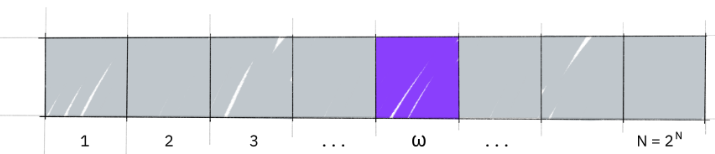
\includegraphics[scale=.6]{Imagens/markedItem.png}\\
    {\small Fonte: Github/\emph{Qiskit}}
    \label{fig:itemMarcado}
\end{figure}

Aqui tem-se ilustrado um conjunto contendo $N = 2^n$ elementos organizados aleatoriamente. Nele, h\'{a} um termo $\omega$ destacado, nomeado "\textit{winner}", que \'{e} justamente o elemento procurado. Se quisesse-se buscar o item marcado por meio de computaç\~{a}o cl\'{a}ssica, seriam necess\'{a}rias, em m\'{e}dia, $\frac{N}{2}$ iterações, contudo, ao implementarmos o Algoritmo de Grover, esse valor cai para $\sqrt{N}$, que \'{e} um avanço significativo, principalmente quando considera-se manipular conjuntos com grandes quantidades de itens \cite{qiskit_GroverNotebook}.

\subsection{Estrutura}
\label{subsec:estruturaAlg}

Para que seja poss\'{i}vel compreender a atuaç\~{a}o do algoritmo, \'{e} preciso entender sua estrutura, que conta com tr\^{e}s partes necess\'{a}rias para que possa ser implementado, sendo elas: preparaç\~{a}o inicial do estado, determinaç\~{a}o do Or\'{a}culo (marcaç\~{a}o do estado buscado) e amplificaç\~{a}o da amplitude e probabilidade (aplicaç\~{a}o do Operador de Grover ou Operador de Difus\~{a}o). Isso pode ser exemplificado pelo esquema da Figura~\ref{fig:groverEsquema}.

\begin{figure}[ht!]
    \centering
    % \captionsetup{justification=centering}
    \caption{Esquematizaç\~{a}o da estrutura do Algoritmo de Grover.}
    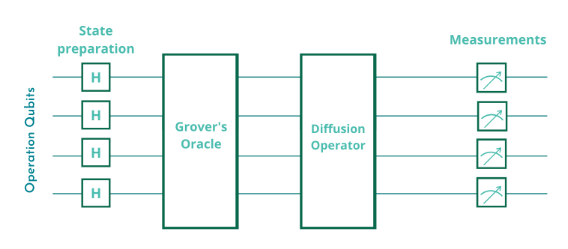
\includegraphics[width=.7\textwidth]{Imagens/esquemaG.png}\\
    {\small Fonte: Github/\emph{Qiskit}.}
    \label{fig:groverEsquema}
\end{figure}

Na preparaç\~{a}o do estado h\'{a} a criaç\~{a}o do que chamaremos de espaço de pesquisa, \'{e} o conjunto que cont\'{e}m o elemento marcado e onde ele ser\'{a} procurado. 

Feito isso, seguiremos para a determinaç\~{a}o do item que queremos encontrar, que \'{e} feita pelo Or\'{a}culo. A atuaç\~{a}o do Or\'{a}culo consiste em inverter a fase do elemento de interesse, ou seja, ele marca o item buscado. Caso haja mais de um item de interesse, o Or\'{a}culo deve agir em todos eles, marcando-os, de modo que sejam destacados pelo difusor.

Por fim, utiliza-se o Operador de Difus\~{a}o para aumentar a amplitude do estado marcado, enquanto decresce as demais, sendo assim uma garantia de que na medida final, o resultado obtido seja aquele procurado.

% \subsection{Funcionamento}
% \label{subsec:funcionamentoAlg}
Quando trabalha-se com o Algoritmo de Grover, pode-se reduzir o problema a um espaço de duas dimensões, sendo necess\'{a}rio considerar apenas o estado buscado -- \textit{winner}, $\ket{\omega}$ --, e a superposiç\~{a}o uniforme, $\ket{s}$. Contudo, esses n\~{a}o s\~{a}o vetores perpendiculares entre si, uma vez que $\ket{\omega}$ ocorre em superposiç\~{a}o com amplitude $\frac{1}{\sqrt{N}}$. Para contornar isso, cria-se um vetor $\ket{s'}$ que \'{e} perpendicular a $\ket{\omega}$, formando assim o plano bidimensional apresentado na Figura~\ref{subfig:Plano}. Na Figura~\ref{subfig:Amplitude}, est\~{a}o ilustradas as amplitudes dos itens contidos no conjunto, evidenciando o elemento \textit{winner}.

\begin{figure}[ht!]
    \centering
    \caption{Plano Bidimensional e Amplitude dos estados da base.}
    \label{fig:espacoAmplitude}
    \begin{subfigure}[b]{0.4\textwidth}
        \centering
        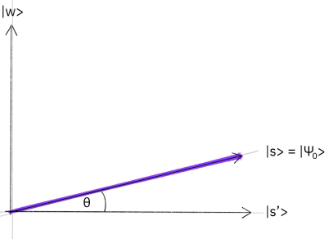
\includegraphics[width=\textwidth]{Imagens/BidimensionalEspaco.png}
        \caption{Plano formado pelos vetores $\ket{\omega}$ e $\ket{s'}$.}
        \label{subfig:Plano}
    \end{subfigure}
    \hfill
    \begin{subfigure}[b]{0.45\textwidth}
        \centering
        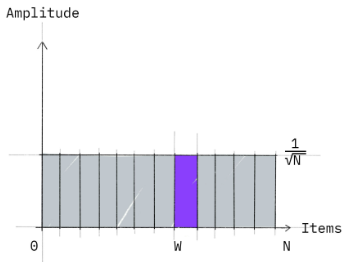
\includegraphics[width=\textwidth]{Imagens/AmplitudesW.png}
        \caption{Amplitude dos itens do conjunto, com $\ket{\omega}$ em destaque.}
        \label{subfig:Amplitude}
    \end{subfigure}

    \vspace{0.3em}
    {\small Fonte: Github/\emph{Qiskit}.}
\end{figure}


% Uma vez introduzida a vis\~{a}o geral sobre como o algoritmo atua, pode-se passar para o estudo de cada uma de suas tr\^{e}s etapas.

%%%%%%%%%%%%%%%%%%%%%%%%%%%%%%%%%%%%%%%%%%%%%%%%%%%%%%%%%%%%%%%%%%%%%%%%%%%%%%%%%%

\subsection{Preparaç\~{a}o Inicial}
\label{subsec:prepInicialAlg}

A Preparaç\~{a}o Inicial \'{e} a etapa inicial do algoritmo, na qual o Espaço de Pesquisa \'{e} criado, matematicamente descrito como uma superposiç\~{a}o uniforme e pela Equaç\~{a}o~\ref{eq:superposicao}, e possui tamanho dado por $N = 2^n$, com $n$ sendo o n\'{u}mero de qubits.

\begin{equation}
    \ket{s} = \frac{1}{\sqrt{N}}\sum_{x = 0}^{N - 1} \ket{bin(x)},
    \label{eq:superposicao}
\end{equation}
%
com $x \in \left\{ 0, 1, 2, \ldots, N-1 \right\}$.

Se uma mediç\~{a}o for realizada na base $\ket{x}$, de acordo com o Quinto Postulado da Mec\^{a}nica Qu\^{a}ntica \cite{vonNuemann1955_QuMec}, a superposiç\~{a}o colapsa, podendo resultar em qualquer um dos estados de mesma probabilidade $\frac{1}{N} = \frac{1}{2^n}$. 

Em termos de circuito qu\^{a}ntico, a superposiç\~{a}o explicitada pela Equaç\~{a}o~\ref{eq:superposicao} pode ser constru\'{i}da facilmente aplicando a porta Hadamard em cada um dos qubits, que se iniciam no estado fundamental $\ket{0}$, como representado pela Equaç\~{a}o~\ref{eq:preparacaoInicial}.
%
\begin{equation}
    \ket{s} = H^{\otimes n}~\ket{0}^n
    \label{eq:preparacaoInicial}
\end{equation}

O vetor $\ket{s}$ que aparece na Figura~\ref{subfig:Plano} pode ser escrito em coordenadas polares, como
%
\begin{equation}
    \ket{s} = \sin{\theta}\ket{\omega} + \cos{\theta}\ket{s'},
    \label{eq:estadoCoordPolar}
\end{equation}

em que 
%
\begin{equation}
    \theta = \arcsin{\braket{s|\omega}} = \arcsin{\frac{1}{\sqrt{N}}}
    \label{eq:thetaValue}
\end{equation}

\subsection{Or\'{a}culo ($U_f$)}
\label{subsec:oraculoAlg}

Tomando a premissa de que o elemento $\omega$ procurado está em um determinado conjunto contendo $N = 2^n$ itens, ${0, 1, 2, ..., N-1}$, com $n \in \mathbb{N}$, podemos recorrer a uma função $f : {0, 1, 2, ..., N-1},\\ \to {1,-1}$ que atua na amplitude dos elementos para marcar o buscado, sendo $f$ tal que
%
\begin{equation}
    f(x) = 
    \begin{cases}
        -1, & \text{se } x = \omega \\
        1, & \text{se } x \neq \omega
    \end{cases}
    \label{eq:fx Oraculo}
\end{equation}

Em outras palavras, o Oráculo, denotado por \simboloinline{$U_f$}{Operador Oráculo}, nada mais é que uma função que gera a reflexão em um \^{a}ngulo $\theta$ de $\ket{s}$ sobre $\ket{s'}$, bem como a reflexão da amplitude do elemento de interesse $\ket{\omega}$, que pode ser visualizado com a ajuda da Figura~\ref{fig:rotacaoReflexao}.

\begin{figure}[ht!]
    \centering
    \captionsetup{justification=centering}
    \caption{Reflexão dos estados $\ket{s}$ e $\ket{\omega}$, respectivamente.}

    \begin{subfigure}[b]{0.4\textwidth}
        \centering
        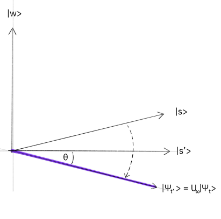
\includegraphics[width=\textwidth]{Imagens/rotacao.png}
        \caption{Reflexão de $\ket{s}$ sobre $\ket{s'}$ em um \^{a}ngulo $\theta$.}
        \label{subfig:rotacao}
    \end{subfigure}
    \hfill
    \begin{subfigure}[b]{0.45\textwidth}
        \centering
        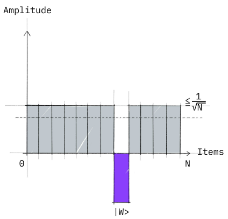
\includegraphics[width=\textwidth]{Imagens/reflexao.png}
        \caption{Reflexão de $\pi$ rads na amplitude de $\ket{\omega}$.}
        \label{subfig:reflexao}
    \end{subfigure}

    \vspace{0.5em}
    {\small Fonte: Github/\emph{Qiskit}.}
    \label{fig:rotacaoReflexao}
\end{figure}


De modo geral, a construção dos Oráculos no Algoritmo de Grover pode ser realizada utilizando portas lógicas qu\^{a}nticas do tipo $X$ e \simboloinline{$MCZ$}{\textit{Porta Lógica Quântica Z-multi-controlada}}, seguindo a seguinte regra de formação:

\begin{enumerate}
\label{enum: regraFormacaoOraculo}
    \item Para cada qubit cujo valor no estado buscado seja $\ket{0}$, aplica-se uma porta $X$ nesse qubit, realizando assim um \textit{bit-flip};
    
    \item Em seguida, aplica-se uma porta ($MCZ$) sobre todos os qubits, marcando o estado desejado com um fator de fase;
    
    \item Por fim, aplica-se novamente a porta $X$ nos mesmos qubits que sofreram o \textit{bit-flip} na primeira etapa, revertendo as alterações realizadas inicialmente.
\end{enumerate}

\subsection{Operador de Difus\~{a}o ($U_s$)}
\label{subsec:difusaoAlg}

A  aplicação do Operador de Difusão, denotado por \simboloinline{$U_s$}{\textit{Operador de Difus\~{a}o}}, consiste em operações de amplificação sobre o estado $\ket{s}$, gerando uma reflexão adicional do mesmo.
%
\begin{equation}
    U_s = 2~\ket{s}\bra{s} - I
    \label{eq:Us}
\end{equation}

Essa transformação mapeia o estado de $\ket{s}$ para $(U_sU_f)\ket{s}$ e completa a transformação, tal como está apresentado na Figura~\ref{fig:transformacaoCompleta}.

\begin{figure}[ht!]
    \centering
    \captionsetup{justification=centering}
    \caption{Segunda reflexão dos estados $\ket{s}$ e $\ket{\omega}$, respectivamente.}
    \label{fig:transformacaoCompleta}  % Label principal após caption

    \begin{subfigure}[b]{0.4\textwidth}
        \centering
        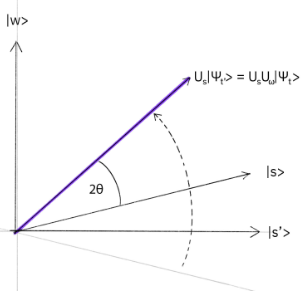
\includegraphics[width=\textwidth]{Imagens/reflexaoEstado.png}
        \caption{Segunda reflexão de $\ket{s}$ sobre $\ket{s'}$.}
        \label{subfig:reflexaoEstado}
    \end{subfigure}
    \hfill
    \begin{subfigure}[b]{0.48\textwidth}
        \centering
        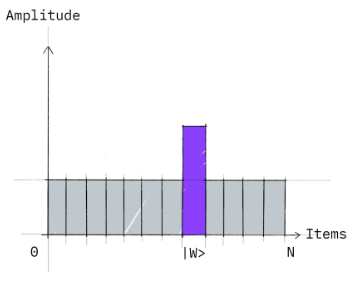
\includegraphics[width=\textwidth]{Imagens/reflexaoAmplitude.png}
        \caption{Segunda reflexão na amplitude de $\ket{\omega}$.}
        \label{subfig:reflexaoAmplitude}
    \end{subfigure}

    \vspace{0.5em}
    {\small Fonte: Github/\emph{Qiskit}.}
\end{figure}

Duas reflexões sempre resultam em uma rotação, que leva o estado inicial $\ket{s}$ para mais perto do elemento \textit{winner}, $\ket{\omega}$. 

Como esta é uma reflexão sobre $\ket{s}$, busca-se adicionar uma fase negativa a cada estado ortogonal a $\ket{s}$. A maneira como pode-se fazer isso é aplicar uma transforma\~{a}o que leva o estado $\ket{s} \to \ket{0}$, com isso, em vez de $U_s$, chamar-se-á $U_0$. Dessa forma, a Equaç\~{a}o~\ref{eq:Us} se torna: 
%
\begin{equation}
    U_0 = 2~\ket{0}\bra{0} - I
    \label{eq:Uo}
\end{equation}

Essa operação aplica uma fase negativa a todos os estados ortonormais a $\ket{0}$, como será demonstrado.

[TALVEZ COLOCAR NUM APÊNDICE***]

Aplicação do Operador $U_0$ em $\ket{s}$, com $\ket{s}$ podendo ser um conjunto arbitr\'{a}rio com $N-1$ itens:

\begin{equation*}
U_0~\ket{s} = \left(2\ket{0}\bra{0} - I\right) \frac{1}{\sqrt{N}}\sum_{x=0}^{N-1} \ket{bin(x)},
\end{equation*}

Expandindo, tem-se:

\begin{equation*}
2~\ket{0}\bra{0} \left( \frac{1}{\sqrt{N}}\sum_{x=0}^{N-1} \ket{bin(x)}\right) = \frac{1}{\sqrt{N}}\sum_{x=0}^{N-1} \ket{bin(x)}
\end{equation*}

\begin{equation}
2~\ket{0} \left( \sum_{x=0}^{15} \braket{0|bin(x)}\right) = \sum_{x=0}^{15} \ket{bin(x)}
\label{eq:aplicacaoDifusor 2}
\end{equation}
%
Como $\braket{0|bin(x)} = 1$ apenas se $x = 0$ (enquanto todos os outros termos se tornam $0$),  o único termo que sobrevive é:
%
\begin{equation*}
2\ket{0}{\braket{0|bin(0)}} = 2\ket{bin(0)}
\end{equation*}

Então, em síntese, tem-se:
%
\begin{align}
\notag
U_0~\ket{s} = &2~\ket{bin(0)} - \sum_{x=0}^{N-1} \ket{bin(x)} \\ 
\notag
= &2~\ket{bin(0)} - \ket{bin(0)} - \ket{bin(1)} - \ket{bin(2)} - \dots - \ket{bin(N-1)} \\ 
= &\ket{bin(0)} - \sum_{x=1}^{N-1} \ket{bin(x)}
\label{eq:aplicacaoDifusao}
\end{align}
%
Ou seja, a amplitude $\ket{bin(0)}$ aumenta em relação aos demais que invertem.

Tendo sido demonstrada a forma matemática, passa-se agora para a apresentação da obtenção do circuito qu\^{a}ntico que realiza essa operação. 

O Operador de Difusão em termos de portas lógicas é dado por:
%
\begin{equation}
    U_s = H^{\otimes n}~U_0~H^{\otimes n}
    \label{gate: operadorDifusao}
\end{equation}

Como já visto, a atuação de $U_0$ é aplicar uma fase negativa a todos os estados ortogonais a $\ket{s}$, e, para isso, deve ser realizada a seguinte sequência:

\begin{enumerate}
\label{enum: difusor}
    \item Aplicação de portas $X$ em todos canais para \textit{bit-flip} dos estados;
    \[\ket{00\cdots0} \to \ket{11\cdots1} \]
    \item Aplicação de porta $MCZ$, com alvo no último canal, pois dessa forma o último estado recebe uma inversão de fase;
    \begin{equation}
    MCZ_{[N \times N]}  =
    \begin{bmatrix}
        1 & 0 &  \cdots  & 0\\
        0 & 1 &  \cdots  & 0\\
        \vdots & \vdots & \ddots & \vdots \\
        0 & 0 &  \cdots & -1\\
    \end{bmatrix}_{[N \times N]}
    \label{mtx: gateMCZ}
\end{equation}
    \item Novamente aplica-se portas $X$ para desfazer os \textit{bit-flips}.
    \[\ket{11\cdots1} \to \ket{00\cdots0} \]
\end{enumerate}

Após a última etapa, o resultado obtido é:

\begin{equation*}
    \begin{bmatrix}
        -1 & 0 &  \cdots  & 0\\
        0 & 1 &  \cdots  & 0\\
        \vdots & \vdots & \ddots & \vdots \\
        0 & 0 &  \cdots & 1\\
    \end{bmatrix}_{[N \times N]}
\end{equation*}

Ou seja, existe ainda uma fase global em $U_0$, de modo que o Operador de Difusão, em termos de portas lógicas, é:
\begin{equation}
    U_0 = -X^{\otimes n}~MCZ~X^{\otimes n}
    \label{gate: difusor}
\end{equation}

O trecho de circuito descrito em Equação está mostrado na Figura~\ref{fig:difusor}

\begin{figure}[!htb]
\centering
\caption{Operador de Difus\~{a}o parcial}
\label{fig:difusor} 
\begin{quantikz}
\lstick{$q_0$}       & \gate{X} & \qw      & \ctrl{1}   & \qw       & \gate{X}  & \qw \\
\lstick{$q_1$}       & \gate{X} & \qw      & \ctrl{2}   & \qw       & \gate{X}  & \qw \\
\lstick{$\vdots$}    &~\vdots~  &          &            & \qw       &~\vdots~   & \qw \\
\lstick{$q_{n-1}$}   & \gate{X} & \gate{H} & \gate{X}   & \gate{H}  & \gate{X}  & \qw \\
\lstick{$c: n$}      & \cw      & \cw      & \cw        & \cw       & \cw       & \cw
\end{quantikz}

\vspace{.3em}
{\small Fonte: do autor} 
\end{figure}

Considerando as Equações~\ref{gate: operadorDifusao} e~\ref{gate: difusor}. Tem-se que o Operador de Difusão completo em portas lógicas qu\^{a}nticas são dados pela Equação~\ref{gate: operadorDifusaoCompleto} e pela Figura~\ref{fig:operadorDifusaoCompleto}.

\begin{equation}
    U_s = H^{\otimes n}~X^{\otimes n}~MCZ~X^{\otimes n}~H^{\otimes n}
    \label{gate: operadorDifusaoCompleto}
\end{equation}

Note que a fase negativa não foi acrescentada, pois não precisa ser considerada no circuito qu\^{a}ntico. 

\begin{figure}[!htb]
\centering
\caption{Operador de Difus\~{a}o completo}
\label{fig:operadorDifusaoCompleto} %rotulo para refencia
\begin{quantikz}
\lstick{$q_0$}       & \gate{H} & \gate{X} &          & \ctrl{1} &          & \gate{X} & \gate{H} & \qw \\
\lstick{$q_1$}       & \gate{H} & \gate{X} &          & \ctrl{2} &          & \gate{X} & \gate{H} & \qw \\
\lstick{$\vdots$}    &~\vdots~  &~\vdots~  &          &          &          & ~\vdots~ & ~\vdots~ & \qw \\
\lstick{$q_{n-1}$}   & \gate{H} & \gate{X} & \gate{H} & \gate{X} & \gate{H} & \gate{X} & \gate{H} & \qw \\
\lstick{$c: n$}      & \cw      & \cw      & \cw      & \cw      & \cw      & \cw      & \cw      & \cw
\end{quantikz}

\vspace{.3em}
{\small Fonte: do autor} 
\end{figure}

\subsection{Fator de Otimizac\~{a}o (k)}
\label{subsec:otimizacao k}

Afim de otimizar o resultado, a aplicação do \nameref{subsec:oraculoAlg} e do \nameref{subsec:difusaoAlg} deverão ser executados um número \simboloinline{$k$}{Fator de Otimização do Algoritmo de Grover} de vezes para que o resultado obtido seja o mais próximo possível (com maiores amplitudes e probabilidades) do estado esperado $\ket{\omega}$, e pode ser expresso por
%
\begin{equation}
    \label{eq:psi k}
    \ket{\psi_k} = (U_sU_f)^k\ket{s}
\end{equation}

O número ideal $k$ de iterações necessárias para que $\ket{\omega}$ seja obtido é dado por

\begin{equation}
    k = \frac{\pi}{4}\sqrt{\frac{N}{m}}
    \label{eq:k value}
\end{equation}
%
em que $N$ é o tamanho do espaço de pesquisa, e $m$ é a quantidade de itens procurados.

A Figura~\ref{fig:algoritmoCompleto} mostra um esquema do Algoritmo de Grover completo, evidenciando o Oráculo e o Operador de Difusão.

\begin{figure}[ht!]
    \centering
    \captionsetup{justification=centering}
    \caption{Esquematização do Algoritmo de Grover.}
    \label{fig:algoritmoCompleto}
    
    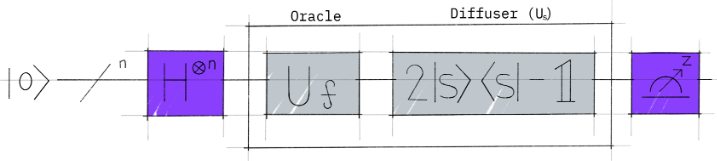
\includegraphics[scale=.5]{Imagens/esquemaAlgG.png}
    
    {\small Fonte: Github/\emph{Qiskit}.}
\end{figure}



\chapter{PROCEDIMENTOS TE\'{O}RICOS E COMPUTACIONAIS}
\label{chap:procedimentos}

Este capítulo descreve detalhadamente os procedimentos teóricos e computacionais adotados para a implementação do Algoritmo de Grover. Inicialmente, apresenta-se o procedimento teórico formalizado matematicamente e expresso por meio de circuitos qu\^{a}nticos compostos por portas lógicas elementares.

Posteriormente, será apresentado o procedimento computacional, que envolve a modelagem e a execução do algoritmo utilizando ferramentas de simulação e programação qu\^{a}ntica. Esta parte tem como objetivo validar teoricamente o funcionamento do algoritmo e analisar, por meio de experimentos práticos, o seu desempenho em ambientes computacionais qu\^{a}nticos. Assim, este capítulo estabelece as bases necessárias para a compreensão e replicação dos resultados obtidos ao longo deste trabalho.

\section{Criando o Circuito Quântico Virtual}
\label{sec: circuitoVirtual}

Nesta seção, serão apresentados de forma integrada os aspectos teóricos e computacionais da implementação do Algoritmo de Grover com $4$ qubits e que orientaram a construção do circuito quântico utilizado no processo. Serão apresentados, também, trechos de código escritos em \emph{Python} utilizando a biblioteca \emph{Qiskit}. A combinação entre fundamentação teórica e simulação computacional permite visualizar com clareza o funcionamento do algoritmo, cujo procedimento foi dividido em três etapas principais:
\begin{enumerate}
    \item a preparação do espaço de pesquisa;
    \item a aplicação do oráculo;
    \item a operação de difusão.
\end{enumerate}

Cada uma dessas etapas é descrita de forma detalhada em uma estrutura que visa garantir clareza na compreensão do funcionamento do circuito e posterior análise dos resultados.

\subsection{Preparação Inicial do Circuito Quântico}
\label{subSec: preparacaoInicialTeo}

A princípio, foi necessário determinar o Espaço de Pesquisa $\ket{s}$, \emph{i. e.}, criar uma superposição uniforme dos estados da base de $4$ qubits. Como sugere a Equação~\ref{eq: superposicao}, para $n=4$ qubits, o Espaço de Pesquisa possui $N = 2^4 = 16$ itens, e é dado por:
%
\begin{align}
    \label{eq: espacoPesquisa}
    \notag
    \ket{s} =&~ \frac{1}{4} \sum_{x=0}^{15} \ket{bin(x)} \\
     =&~ \frac{1}{4} (\ket{0000} +  \ket{0001} +  \ket{0010} +  \ket{0011} +  \ket{0100} +  \ket{0101} +  \ket{0110} + \ket{0111} +  \\
    \notag{}
     &~~~~~\ket{1000} +  \ket{1001} +  \ket{1010} +  \ket{1011} +  \ket{1100} +  \ket{1101} +  \ket{1110} +  \ket{1111})
\end{align}
%
\tab\tab Para a implementação do circuito quântico virtual em \emph{Qiskit}, deve-se primeiramente importar as dependências e instanciar as variáveis do circuito. As dependências relacionadas à biblioteca \emph{Qiskit} são apresentadas na Figura~\ref{cod: dependencias} e a importação e declaração dos recursos na Figura~\ref{cod: inicializacao}.

\begin{figure}[!htb]
\centering
\caption{Dependências do Programa   } 
\begin{minted}{json}
{
  "QiskitDependencies": {
    "qiskit": "2.1.2",
    "qiskit-aer": "0.17.1",
    "qiskit-ibm-provider": "0.11.0",
    "qiskit-ibm-runtime": "0.41.1"
  }
}
\end{minted} 
{\small Fonte: do autor} 
\label{cod: dependencias} 
\end{figure}

\begin{figure}[!htb]
\centering
\caption{Inicialização do Circuito Qu\^{a}ntico} 
\begin{minted}{python}
from qiskit import QuantumCircuit, QuantumRegister, ClassicalRegister

n = <num_qubits>
qubits = QuantumRegister(n, 'qubit')
bits= ClassicalRegister(n, 'bit')

QC_Grover = QuantumCircuit(qubits, bits)
\end{minted} 
{\small Fonte: do autor} 
\label{cod: inicializacao} 
\end{figure}

A Figura~\ref{cod: inicializacao} mostra \verb|QC_Grover|, que é um objeto instanciado pela classe \verb|QuantumCircuit|. Nela será adicionado todo o circuito. Por sua vez, \verb|qubits| e \verb|bits| são instâncias das classes \verb|QuantumRegister| e \verb|ClassicalRegister|, respectivamente, que serão responsáveis pelo armazenamento dos dados e importantes no processo de medição.

A próxima etapa é a formação do espaço de pesquisa mencionado anteriormente e, para isso, pode-se recorrer à Equação~\ref{eq: preparacaoInicial}, que implica no uso de portas $Hadamard$ em cada \emph{qubit}. Esse passo é feito usando o módulo \verb|inicializa_s|, apresentado na Figura~\ref{cod: preparacao}.

\begin{figure}[!htb]
\centering
\caption{Módulo Preparação Inicial} 
\begin{minted}{python}
def inicializa_s(qc, qubits):
    for qubit in qubits:
        qc.h(qubit)
    return qc
\end{minted} 
{\small Fonte: do autor} 
\label{cod: preparacao} 
\end{figure}

Uma representação visual do circuito quântico virtual relativo a este trecho pode ser acompanhada na Figura~\ref{fig: preparacaoInicial}. É relevante notar que todos os \textit{qubits} são inicializados no estado $\ket{0}$.
%
\begin{figure}[!htb]
    \centering
    \caption{Circuito Quântico Virtual - Superposição}
    \label{fig: preparacaoInicial} 
    
    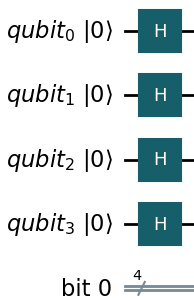
\includegraphics[scale=0.5]{Imagens/preparacaoInicial.png}

    \vspace{0.3em}
    {\small Fonte: do autor} % Fonte da imagem
\end{figure}
%
\subsection{Or\'{a}culo}
\label{subSec: oraculoTeo}

Para dar prosseguimento, é preciso marcar o estado que se deseja obter, \emph{i. e.}, aplicar o \nameref{subSec: oraculoAlg} (Equaç\~{a}o~\ref{eq: fx Oraculo}) ao Espaço de Pesquisa (Equaç\~{a}o~\ref{eq: espacoPesquisa}). Seja $\omega = \ket{1111}$ o estado arbitrariamente escolhido para ser buscado, a aplicação do Oráculo é tal que
%
\begin{align}
    \notag
    U_f\ket{s} = ~& \frac{1}{4}~U_f~[\ket{0000} + \ket{0001} + \ket{0010} + \ket{0011} + \ket{0100} + \ket{0101} + \ket{0110} +\ket{0111} + \\ \notag
    &~ \ket{1000} + \ket{1001} + \ket{1010} + \ket{1011} + \ket{1100} + \ket{1101} + \ket{1110} + \ket{1111}] \\
    \label{eq: aplicacaoOraculo}
    = &~ \frac{1}{4}(\ket{0000} + \ket{0001} + \ket{0010} + \ket{0011} + \ket{0100} + \ket{0101} + \ket{0110} +\ket{0111} + \\ \notag
    &~ \ket{1000} + \ket{1001} + \ket{1010} + \ket{1011} + \ket{1100} + \ket{1101} + \ket{1110} + -\ket{1111})
\end{align}
%
Que pode ser expresso de acordo com a matriz $16 \times 16$
%
\begin{equation*}
    (U_{f}~\ket{s})_{[16 \times 16]} = \begin{bmatrix}
        1 & 0 &  \cdots  & 0\\
        0 & 1 &  \cdots  & 0\\
        \vdots & \vdots & \ddots & \vdots \\
        0 & 0 &  \cdots  & -1\\
    \end{bmatrix}_{[16 \times 16]} 
    \label{mtx: aplicacaoOraculo}
\end{equation*}

O desafio seguinte foi determinar a(s) porta(s) lógica(s) que retorna(m) essa matriz. Para isso, pode-se seguir a regra de formação enunciada na Seção~\ref{subSec: oraculoAlg} do Capítulo~\nameref{chap: ferramentas}. Como o estado buscado é $\omega = \ket{1111}$, não será necessário o uso de portas $X$, apenas uma $MCZ$ (Equação~\ref{mtx: gateMCZ}) será suficiente, pois o resultado prático que se obtém com a aplicação da porta $MCZ$ é basicamente mudar a fase do último elemento da matriz $N \times N$ à qual ela for aplicada, exatamente o que se intenta obter; portanto, o Oráculo será uma porta $MCZ$.

Em \emph{Qiskit}, a implementação é feita com o módulo \verb|oraculo_Uw|, mostrado na Figura~\ref{cod: oraculo}. E o circuito quântico virtual relativo a este trecho é mostrado na Figura~\ref{fig: aplicacaoOraculo}\footnote
{
Como o \emph{Qiskit} não oferece suporte nativo à porta $MCZ$, ela é construída combinando portas $Hadamard$ e $MCX$, visto que $MCZ=H~MCX~H$ ($H$'s apenas no qubit alvo).

[TALVEZ DEMONSTRAR NO APÊNDICE***]
}.

\begin{figure}[!thb]
\centering
\caption{Módulo Oráculo} 
\begin{minted}{python}
def mcz_circ(qc):
    qc.h(3)
    qc.mcx([0, 1, 2], 3)
    qc.h(3)
    return qc
    
def oraculo_Uw(qc, qubits, winner, QuantumCircuit):
    for i, index in enumerate(winner):
        if index == "0":
            qc.x(i)

    # Para agrupar as portas H MCX H em uma MCZ
    mcz_gate = mcz_circ(qc = QuantumCircuit(4,name="mcz")).to_instruction() 
    qc.append(mcz_gate,[i for i in range(4)])

    for i, index in enumerate(winner):
        if index == "0":
            qc.x(i)
\end{minted} 
{\small Fonte: do autor} 
\label{cod: oraculo} 
\end{figure}

O módulo \verb|mcz_circ| apenas é usado para agrupar o conjunto de portas $H~MCX~H$ em um único bloco, para facilitar identificação. Para fins de ilustração, vide Figura~\ref{fig: aplicacaoOraculo}. O parâmetro \texttt{winner} representa o estado marcado a ser identificado (por exemplo, $\ket{1111}$).

\begin{figure}[!htb]
    \centering
    \captionsetup{justification=centering}
    \caption{Circuito Quântico Virtual - Oráculo}
    \label{fig: aplicacaoOraculo}

    \begin{subfigure}[b]{0.16\textwidth}
        \centering
        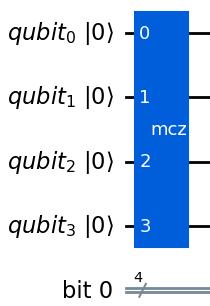
\includegraphics[width=\textwidth]{Imagens/oraculoContraido.png}
        \caption{Oráculo contraído.}
        \label{subfig: oraculoContraido}
    \end{subfigure}
    \hspace{1cm}
    \begin{subfigure}[b]{0.25\textwidth}
        \centering
        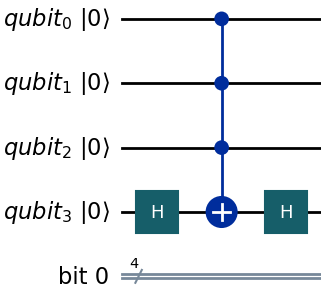
\includegraphics[width=\textwidth]{Imagens/oraculoExpandido.png}
        \caption{Oráculo expandido.}
        \label{subfig: oraculoExpandido}
    \end{subfigure}

    \vspace{0.3em}
    {\small Fonte: do autor.}
\end{figure}
%
\subsection{Difus\~{a}o}
\label{subSec: difusaoTeo}

A etapa seguinte é a de amplificação do estado buscado, aplicando uma segunda reflexão $U_s$ (Equaç\~{a}o~\ref{eq:Us}) na resultante da etapa anterior. Conforme demonstrado na Seção~\ref{subsec:difusaoAlg}, Capítulo~\nameref{chap: ferramentas}, a operação que se deseja realizar é dada pela Equação~\ref{eq:aplicacaoDifusao}. Essa operação aplica uma fase negativa a todos os estados ortonormais a $\ket{0}$, \emph{i. e.}, a expansão da Equação~\ref{eq:aplicacaoDifusao} para quatro qubits resulta em:

\begin{equation}
U_0~\ket{s} = \ket{0000} - \ket{0001} - \ket{0010} - \ket{0011} - \cdots - \ket{1111} 
\end{equation}

Ou seja, a amplitude $\ket{0000}$ aumenta em relação aos demais que invertem.

O difusor é representado pela matriz:

\begin{equation}
U_0 = -
\begin{pmatrix}
-1 & 0 & \cdots & 0 \\
0 & 1 & \cdots & 0 \\
\vdots & \vdots & \ddots & \vdots \\
0 & 0 & \cdots & 1
\end{pmatrix}
\label{mtx: Difusao}
\end{equation}

Para colocar isso em termos de portas lógicas, basta utilizar o conjunto de portas apresentado pela Equação~\ref{gate: operadorDifusaoCompleto}. Em \emph{Qiskit}, a implementação pode ser feita com o uso do módulo \verb|difusor_Us|, visto na Figura~\ref{cod: difusao}.

\begin{figure}[!hb]
\centering
\caption{Módulo Operador de Difusão} 
\begin{minted}{python}
def difusor_Us(qc, qubits):
    for i in qubits:
        qc.h(i)
        qc.x(i)

    # Para agrupar as portas H MCX H em uma MCZ
    mcz_gate = mcz_circ(qc = QuantumCircuit(4,name="mcz")).to_instruction() 
    qc.append(mcz_gate,[i for i in range(4)])

    for i in qubits:
        qc.x(i)
        qc.h(i)
    return qc
\end{minted} 
{\small Fonte: do autor} 
\label{cod: difusao} 
\end{figure}

A idealização virtual desse trecho pode ser observada na Figura~\ref{fig: difusaoCompleto}. Nela, é possível fazer a equivalência entre $U_0$ (Equação~\ref{gate: difusor}) e a Figura~\ref{subFig: Uo} e entre $U_s$ (Equação~\ref{gate: operadorDifusaoCompleto}) e a Figura~\ref{subFig: Us}.
%
\begin{figure}[ht!]
    \centering
    \captionsetup{justification=centering}
    \caption{Circuito Qu\^{a}ntico Virtual - Amplificação, $U_0$ e $U_s$.}
    \label{fig: difusaoCompleto}

    \begin{subfigure}[b]{0.25\textwidth}
        \centering
        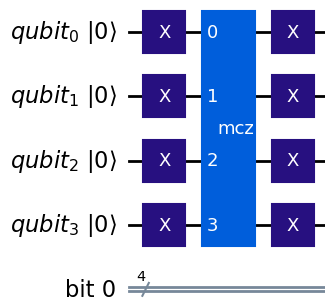
\includegraphics[width=\linewidth]{Imagens/circuitoDifusor.png}
        \caption{Circuito de $U_0$}
        \label{subFig: Uo}
    \end{subfigure}
    \hspace{1cm}
    \begin{subfigure}[b]{0.35\textwidth}
        \centering
        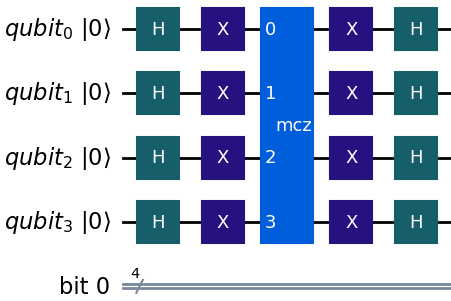
\includegraphics[width=\linewidth]{Imagens/circuitoDifusorCompleto.png}
        \caption{Circuito de $U_s$}
        \label{subFig: Us}
    \end{subfigure}
    
    \vspace{0.3em}
    {\small Fonte: do autor} 
\end{figure}

\subsection{Fator \emph{k}}

Para que a Equação~\ref{eq:psi k} seja de fato satisfeita, deve-se determinar o fator de otimização, \emph{i. e.}, a quantidade de vezes que o \nameref{subsec:oraculoAlg} e o \nameref{subsec:difusaoAlg} devem ser repetidos. O valor de $k$ pode ser obtido com a utilização da Equação~\ref{eq:k value}, em que tem-se $N=16$ e $m=1$.
%
\begin{align*}
    k =&~ \frac{\pi}{4}\sqrt{\frac{N}{m}}\\
    =&~ \frac{\pi}{4}\sqrt{16}\\
    =&~ \pi
\end{align*}
E como $k$ não pode ser número de ponto flutuante, deve-se arredondar para o inteiro mais próximo, ou seja, para fins práticos,
\begin{equation}
    k = 3
    \label{eq: k = 3}
\end{equation}.
Nesse ponto, tem-se que todas as etapas estão concluídas, cabendo, então, uní-las em um único circuito qu\^{a}ntico. Em \emph{Qiskit}, isso pode ser feito com o trecho de código mostrado na Figura~\ref{cod: geraCircuitoCompleto}, que leva em consideração o valor de $k$, por meio de um \textit{loop} \verb|for| no intervalo dado por $k$. Ao final, aplica-se o método \verb|measure()| ao circuito, que realiza a medição dos \textit{qubits}, colapsando o sistema em um dos estados da base computacional, revelando o resultado da busca.

\begin{figure}[!htb]
\centering
\caption{Trecho para formação do Circuito Quântico Virtual.} 
\begin{minted}{python}
N = 2**n
k = (round((pi/4)*sqrt(N)))
marked_state = "<seu_estado>"
inicializa_s(QC_Grover, range(n))

for _ in range(k):
    QC_Grover.barrier([i for i in range(n)])
    oraculo_Uw(QC_Grover, range(n), marked_state, QuantumCircuit)
    difusor_Us(QC_Grover, (range(n)))

QC_Grover.barrier([i for i in range(n)])
QC_Grover.measure([0,1,2,3],[0,1,2,3])
\end{minted} 
{\small Fonte: do autor} 
\label{cod: geraCircuitoCompleto} 
\end{figure}

O circuito relativo ao trecho em questão pode ser visto na Figura~\ref{fig: circuitoCompleto}. As barreiras (\texttt{barrier()}), nesse caso, são apenas separadores visuais do processo de iteração, e os objetos ao final de cada canal indicam o processo de medição do estado final sendo armazenado nos canais clássicos.

\begin{figure}[!thb]
    \centering
    \captionsetup{justification=centering}
    \caption{Circuito Quântico Virtual - Algoritmo de Grover Completo.}
    \label{fig: circuitoCompleto}
    
    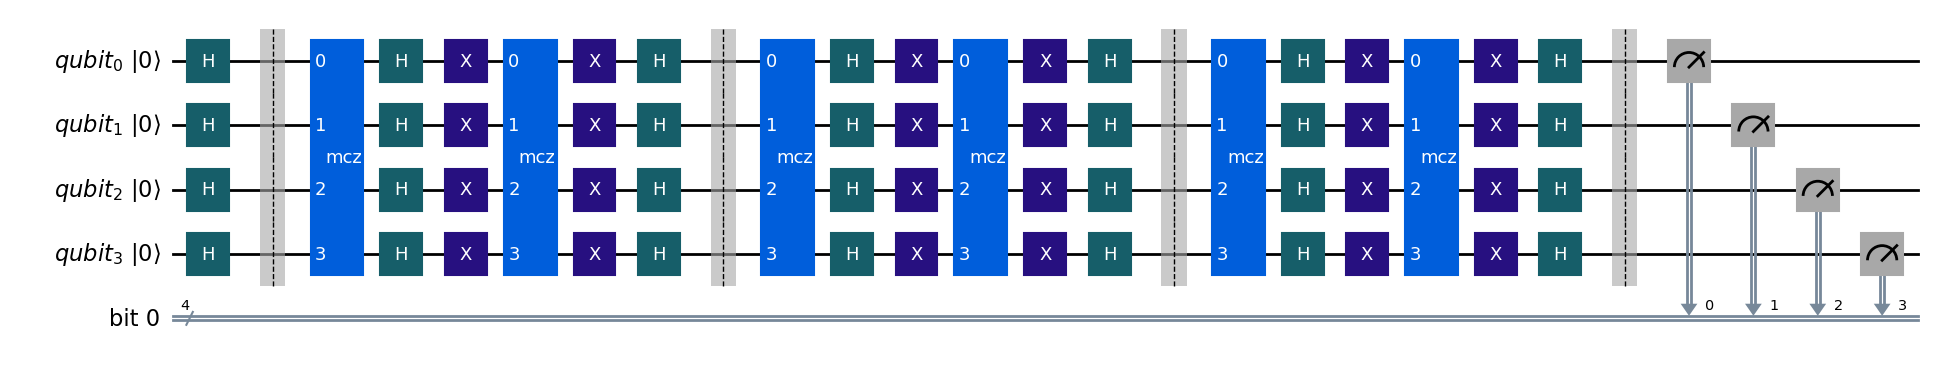
\includegraphics[width=\linewidth]{Imagens/circuitoCompleto.png}

    \vspace{0.1em}
    {\small Fonte: do autor} 
\end{figure}
\section{Plataforma \textit{IBM Quantum}}
\label{sec: plataformaIBM}

Nesta seção, descreve-se e elucida-se por meio de trechos de códigos exemplos o procedimento adotado para o acesso e preparação da simulação do circuito do Algoritmo de Grover utilizando os recursos computacionais da \textit{IBM Quantum Platform} \cite{IBM_quantum}. Essa plataforma online desenvolvida pela IBM permite a execução de algoritmos em computadores quânticos reais e simuladores avançados disponíveis na nuvem.

O primeiro passo consiste na criação de uma conta na plataforma e posterior autenticação com uma organização habilitada. Dentro do ambiente web, o usuário pode configurar projetos e acessar diferentes dispositivos quânticos, incluindo simuladores ideais (sem ruído), simuladores com ruído e \textit{hardwares} reais. Cada projeto está vinculado a uma \textit{instância}, que define os recursos disponíveis, como prioridade de fila e acesso a dispositivos específicos.

Diferentemente dos ambientes locais de simulação, como os disponíveis via \texttt{AerSimulator} no \textit{Qiskit}, a \textit{IBM Quantum} exige que até mesmo as simulações ideais sejam submetidas remotamente, exigindo autenticação prévia e conexão à nuvem. Com a migração da plataforma para o novo modelo unificado, o canal de acesso deve ser definido como \verb|ibm_quantum_platform|, e é obrigatória a definição explícita da \textit{instância}.

\subsection{Procedimento de Autenticação}
\label{subSec: auth}

A seguir, a Figura~\ref{cod: acessaIBM} apresenta um exemplo do código utilizado para salvar e autenticar uma conta na plataforma, utilizando a biblioteca \verb|qiskit_ibm_runtime|:

\begin{figure}[!htb]
\centering
\caption{Trecho de acesso à \textit{IBM Quantum Platform}.} 
\begin{minted}{python}
from qiskit_ibm_runtime import QiskitRuntimeService

QiskitRuntimeService.save_account(
    token="<seu_token>",
    instance="<sua_instancia>",
    channel="ibm_quantum_platform",
    overwrite=True,
    set_as_default=True
)
service = QiskitRuntimeService()
\end{minted} 
{\small Fonte: do autor} 
\label{cod: acessaIBM} 
\end{figure}

O \texttt{token} pode ser obtido no perfil do usuário na plataforma, enquanto a \texttt{instance} segue o padrão \texttt{<hub>/<group>/<project>}, que pode ser consultado no painel de gerenciamento de projetos da \textit{IBM Quantum Platform}. A chamada \verb|set_as_default=True| permite que o serviço seja usado diretamente nos próximos acessos, sem necessidade de repetir a autenticação.

Após essa configuração inicial, torna-se possível listar os dispositivos disponíveis, verificar seus estados (como filas, fidelidades e número de qubits), selecionar o \textit{backend} desejado e submeter os circuitos para execução.

\subsection*{Fluxo de Execução na Nuvem}

O processo completo de execução de um circuito na plataforma envolve:

\begin{itemize}
    \item Construção do circuito com bibliotecas do \texttt{Qiskit};
    \item Escolha do \textit{backend} apropriado (simulador ou QPU);
    \item Submissão da tarefa à nuvem via \texttt{QiskitRuntimeService};
    \item Acompanhamento da execução e análise dos resultados.
\end{itemize}

\subsection{Simulação Ideal via \texttt{Statevector}}
\label{subSec: simulacaoIdeal}

Essa seção traz um exemplo de código que gera uma distribuição de probabilidades ideal, utilizando a classe \texttt{Statevector} do \texttt{Qiskit}, apresentada na Figura~\ref{cod: simulacaoIdeol}, que simula a evolução do estado quântico de forma exata e livre de ruído. Essa abordagem fornece a expectativa teórica para o comportamento do algoritmo de Grover.

\begin{figure}[!htb]
\centering
\caption{Trecho para Simulação Ideal.} 
\begin{minted}{python}
from qiskit.quantum_info import Statevector
ideal_distribution = Statevector.
                     from_instruction(QC_Grover).
                     probabilities_dict()
fig, ax = plt.subplots()
plot_histogram(ideal_distribution, 
               title="Distribuição Ideal de Probabilidades",
               ax=ax)
ax.set_ylabel("Probabilidade")
plt.show()
\end{minted}
{\small Fonte: do autor} 
\label{cod: simulacaoIdeol} 
\end{figure}

Este resultado serve como referência teórica da máxima fidelidade, permitindo a comparação com as demais execuções e a análise da influência dos ruídos nos sistemas quânticos reais.

\subsection{Simulação com Ruído via \textit{AerSimulator}}
\label{subSec: simulacaoRuido}

Essa seção apresenta uma simulação mais próxima da realidade, pois faz uso de informações de ruído da QPU escolhida (definindo \texttt{<nome\_backend>}). Para isso, utiliza a classe \texttt{AerSimulator}, da biblioteca \texttt{qiskit\_aer}. O código exemplo é mostrado na Figura~\ref{cod: simulacaoRuido}. Essa é uma forma de criar uma simulação que busca imitar de forma mais precisa o comportamento prático do circuito, uma vez que a simulação com ruído permite observar a degradação de fidelidade causada por imperfeições reais nos dispositivos quânticos.

\begin{figure}[!htb]
\centering
\caption{Trecho para Simulação com Ruído.} 
\begin{minted}{python}
from qiskit_aer import AerSimulator
from qiskit.compiler import transpile

service = QiskitRuntimeService()
backend = service.backend('<nome_backend>')

# Gerar simulador com modelo de ruído real
backend_sim = AerSimulator.from_backend(backend)
transpiled_circ_sim = transpile(QC_Grover, backend_sim)
result = backend_sim.run(transpiled_circ_sim, shots=<num_shots>).result()
circuits.append(transpiled_circ_sim)
\end{minted}
{\small Fonte: do autor} 
\label{cod: simulacaoRuido} 
\end{figure}

Essa abordagem é valiosa para testar e validar circuitos antes da submissão ao \textit{hardware} físico, permitindo ajustes e observação de efeitos de ruído específicos, como erros de porta, leitura e decoerência.

\subsection{Execução em  via \texttt{Sampler}}
\label{subSec: execucaoQPU}

Por fim, essa última seção traz os procedimentos a serem realizados para a execução em uma QPU. Antes de o circuito ser enviado a alguma QPU propriamente dita, ele precisa ser reescrito em uma linguagem que ela entenda, \textit{i. e.}, o circuito virtual precisa ser reescrito em termos das portas base do \textit{backend} no qual se pretende enviá-lo. Essa é a etapa de compilação mencionada na Seção~\ref{subSec: computadores} e sua implementação é feita com a função \texttt{transpile} conforme mostrado na Figura~\ref{cod: compilacao}.

\begin{figure}[!htb]
\centering
\caption{Trecho para Compilação.} 
\begin{minted}{python}
from qiskit.compiler import transpile

backend_HW = service.backend("<nome_backend>")
transpiled = transpile(QC_Grover, backend_HW, optimization_level=<optim_lvl>)
\end{minted}
{\small Fonte: do autor} 
\label{cod: compilacao} 
\end{figure}

A definição de <\texttt{nome\_backend}> é o que garante a compilação ideal de acordo com as portas base de cada \textit{backend}, visto que cada tipo de processador pode possuir portas base diferentes. Pode-se também configurar o nível de otimização, explanado na Seção~\ref{subSubSec: otimizacao}, por meio de \texttt{optimization\_level}. Concluída essa etapa, segue-se com o circuito compilado.

A Figura~\ref{cod: execucaoSampler} mostra um trecho de exemplo para execução em QPU's que possibilita também utilizar as técnicas de supressão -- \textit{Dynamical Decoupling} (DD) e \textit{Pauli Twirling} introduzidas na Seção~\ref{subSec: supressao} -- disponíveis na classe \texttt{Sampler} da biblioteca \texttt{qiskit\_ibm\_runtime}.

\begin{figure}[!htb]
\centering
\caption{Trecho para Execução em QPU via \texttt{Sampler}.} 
\begin{minted}{python}
from qiskit_ibm_runtime import SamplerV2 as Sampler, Batch

def rodar():
    num_shots = <num_shots>
    with Batch(backend=backend_HW):
        sampler = Sampler()
        # Execução com Dynamical Decoupling + Pauli Twirling
        sampler.options.dynamical_decoupling.enable = True
        sampler.options.twirling.enable_gates = True
        job_DD_Twiling = sampler.run([transpiled], shots=num_shots)
try:
    rodar()
except Exception as e:
    print(f"Erro: {e}")
\end{minted}
{\small Fonte: do autor} 
\label{cod: execucaoSampler} 
\end{figure}

A Figura~\ref{cod: execucaoEstimate}, por sua vez, mostra um trecho de exemplo para execução em QPU's que possibilita utilizar as técnicas de mitigação -- \textit{Twirled Readout Error eXtinction} (TREX), \textit{Zero-Noise Extrapolation} (ZNE), \textit{Probabilistic Error Amplification} (PEA), e \textit{Probabilistic Error Cancellation} (PEA) introduzidas na Seção~\ref{subSec: mitigacao} -- disponíveis na classe \texttt{Estimate} da biblioteca \texttt{qiskit\_ibm\_runtime}.

\begin{figure}[!htb]
\centering
\caption{Trecho para Execução em QPU via \texttt{Estimate}.} 
\begin{minted}{python}

COLOCAR CODIGO COM ESTIMATE***

\end{minted}
{\small Fonte: do autor} 
\label{cod: execucaoEstimate} 
\end{figure}

A execução real permite não apenas verificar a eficiência do algoritmo em ambiente prático, mas também comparar os efeitos das técnicas de supressão aplicadas, ajudando a entender o comportamento dos sistemas quânticos sob influência de ruído quântico.



\input{Secoes/ExecucaoQC}


\chapter{Resultados e Análise}
\label{chap: resultados}

Este capítulo apresentará os resultados obtidos com a execução do Algoritmo de Grover em diferentes contextos computacionais: simulação ideal, simulação com ruído e execução real em hardware quântico. Os resultados são apresentados na forma de gráficos de distribuição de probabilidades dos estados finais, permitindo comparações qualitativas e quantitativas entre os cenários.

\section{Resultado Ideal (Teórico)}
\label{sec: resultIdeal}

Nesta seção, são apresentados os resultados obtidos a partir da simulação teórica ideal do circuito do Algoritmo de Grover, tal qual exemplificado na Figura~\ref{cod: simulacaoIdeol} da Seção~\ref{subSec: simulacaoIdeal}. Esta simulação permite visualizar a distribuição de probabilidades do estado final de maneira exata e sem influência de ruídos externos, funcionando como uma referência teórica para as demais simulações.

A Figura~\ref{fig: resultIdeal} mostra o histograma gerado após a aplicação do algoritmo, considerando um circuito com $4$ qubits e o estado marcado $\omega = \ket{1111}$. Observa-se que o algoritmo amplifica significativamente a probabilidade de ocorrência do estado marcado, como era esperado teoricamente.

\begin{figure}[ht!]
    \centering
    \captionsetup{justification=centering}
    \caption{ Distribuição Ideal de Probabilidades (Simulação via \texttt{Statevector}).}
    \label{fig: resultIdeal}
    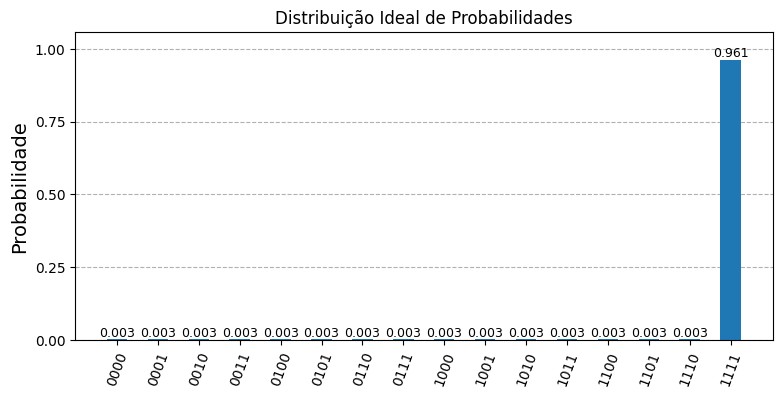
\includegraphics[width=.5\linewidth]{Imagens/resultIdeal.png}    
    
    {\small Fonte: do autor} 
\end{figure}

Com o valor ideal de iterações $k=3$ (resultado~\ref{eq: k = 3}), a probabilidade de medir o estado marcado $\ket{1111}$ foi de $96,1\%$, enquanto os demais estados apresentam probabilidades próximas de zero. Este comportamento é compatível com a expectativa teórica do algoritmo de Grover, conforme discutido nas seções anteriores e demonstrado também no Apêndice~\ref{ap: demonstracaoCircuito}.

A distribuição obtida reflete, portanto, a eficiência máxima do algoritmo quando executado em condições ideais. Esta simulação serve como base de comparação para as análises subsequentes, em que serão incluídos fatores realistas como ruído, erro de leitura e imperfeições físicas presentes nos dispositivos quânticos atuais.

\section{Resultado com Ruído (\texttt{AerSimulator})}
\label{sec: resultRuido}

A simulação ideal apresentada na seção anterior assume um sistema quântico livre de ruídos. No entanto, implementações reais são afetadas por diversos tipos de erros, como decoerência, erro de porta, erro de leitura e ruído térmico. Para aproximar a execução do algoritmo à realidade dos dispositivos quânticos atuais, é necessário considerar esses fatores na simulação.

Esta seção tem por premissa a apresentação dos resultados da simulação feita usando dados de ruídos de dois \textit{backends} diferentes, já mencionados no Quadro~\ref{tab: backends}. Os modelos de ruídos são fornecidos pela classe \texttt{AerSimulator}, e podem ser utilizados como exemplificado na Figura~\ref{cod: simulacaoRuido} da Seção~\ref{subSec: simulacaoRuido}. Este modelo inclui características específicas e atuais do dispositivo real, como fidelidade de portas, taxas de erro de leitura e tempos de decoerência dos qubits, e por isso se faz uma ferramenta valiosa.

A Figura~\ref{fig: resultRuido} mostra o histograma da probabilidade final, em termos de porcentagem, de cada estado.

\begin{figure}[ht!]
    \centering
    \captionsetup{justification=centering}
    \caption{Distribuição de Probabilidades (Simulação via \texttt{AerSimulator}).}
    \label{fig: resultRuido}
    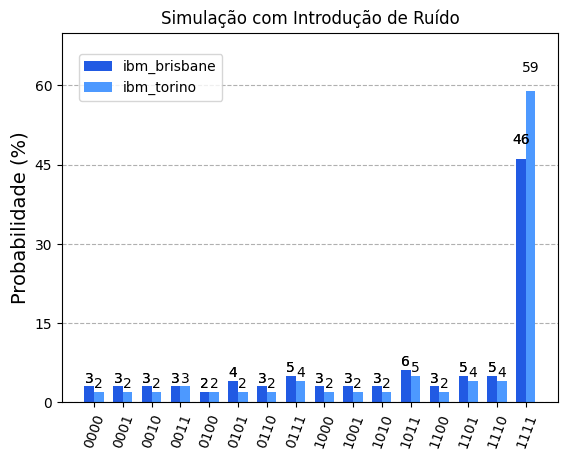
\includegraphics[width=.5\linewidth]{Imagens/resultRuido.png}    
    
    {\small Fonte: do autor} 
\end{figure}

Apesar da presença de ruído, observa-se que o estado marcado $\ket{1111}$ ainda possui a maior probabilidade entre os estados possíveis para ambos os modelos de ruído utilizados, com $46\%$ e $59\%$ para \textit{ibm\_brisbane} e \textit{ibm\_torino}, respectivamente. No entanto, pode-se notar facilmente que a presença do ruído, mesmo em ambiente simulado, já fornece um resultado bastante distorcido com relação à expectativa teórica (ou ideal), na qual a probabilidade para o estado marcado era superior a $96\%$. Ademais, os outros estados apresentam valores não desprezíveis, evidenciando a dispersão causada pelos erros quânticos.

\section{Resultado Real em \textit{Hardware} Quântico (\texttt{Sampler})}
\label{sec: resultReal}

Após a validação teórica e a simulação com ruído, o Algoritmo de Grover foi executado em dois computadores quânticos reais da \textit{IBM Quantum}: \textit{ibm\_brisbane} e \textit{ibm\_torino}, introduzidos na Seção~\ref{subSec: computadores}. A escolha de dois dispositivos teve como objetivo comparar o desempenho do mesmo circuito em arquiteturas físicas distintas, permitindo observar variações de fidelidade e impacto de parâmetros específicos de cada backend.

Para cada execução, foram configurados $20000$ \textit{shots}, e algumas condições específicas, conforme descritas abaixo:

\begin{enumerate}
    \item Sem nenhum método de supressão.
    \item \textit{Dynamical Decoupling} habilitado e \textit{Pauli Twirling} desabilitado.
    \item \textit{Dynamical Decoupling} desabilitado e \textit{Pauli Twirling} habilitado.
    \item Ambos habilitados.
\end{enumerate}

Esse mesmo padrão foi aplicado com dois níveis diferentes de otimização ($2$ e $3$). Todas essas diferentes preparações foram com o intuito de estudo e avaliação dos efeitos de cada método, inclusive quando aplicados simultaneamente.

A apresentação dos resultados é feita baseada nessas configurações, em que pode-se analisar em cada gráfico as diferenças causadas pelos métodos de supressão para um mesmo nível de otimização. Dito isso, a Figura~\ref{fig: resultBrisbane} mostra as quatro configurações de supressão aplicadas aos níveis de otimização $2$ e $3$ (Figuras~\ref{subFig: resultBrisbane_2} e~\ref{subFig: resultBrisbane_3}), enquanto a Figura~\ref{fig: resultTorino} replica as mesmas quatro configurações, também com os dois níveis de otimização aplicados a cada histograma (Figuras~\ref{subFig: resultTorino_2} e~\ref{subFig: resultTorino_3}). 

\begin{figure}[ht!]
    \centering
    \captionsetup{justification=centering}
    \caption{Resultados de \textit{ibm\_brisbane}.}
    \label{fig: resultBrisbane}

    \begin{subfigure}[b]{.46\textwidth}
        \centering
        \caption{Histograma de \textit{ibm\_brisbane} com $optim\_lvl = 2$}
        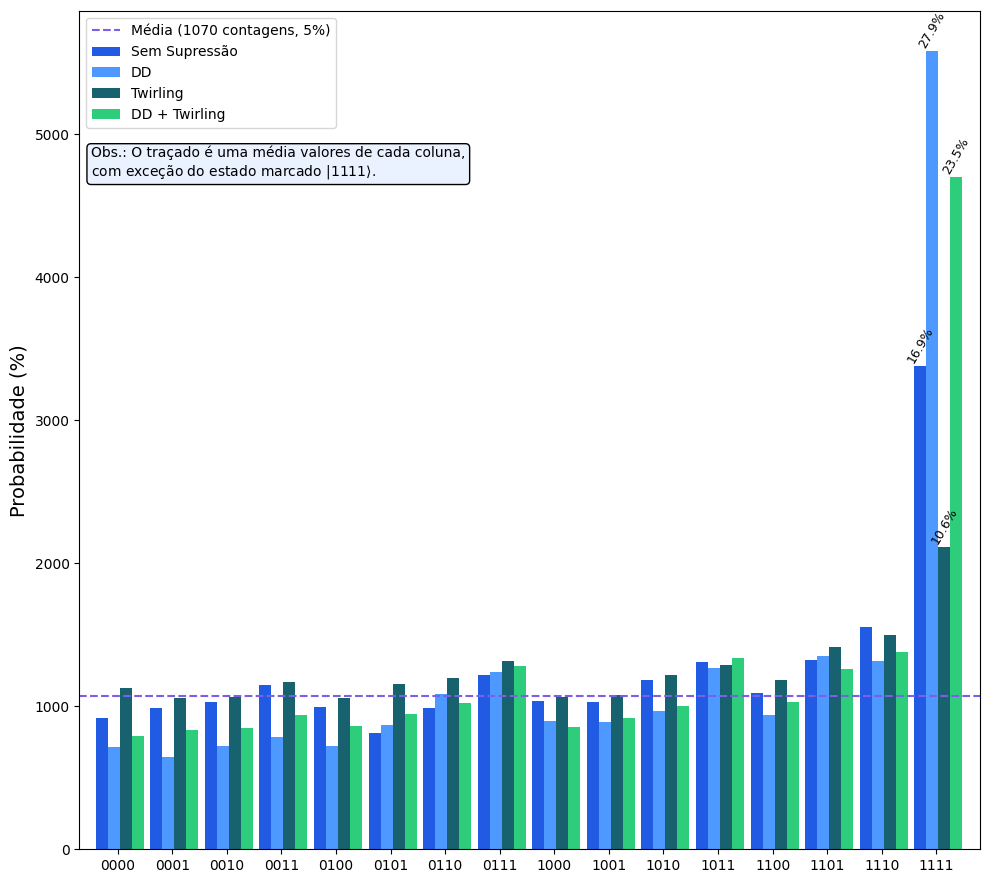
\includegraphics[width=\linewidth]{Imagens/resultBrisbane_2.png}
        \label{subFig: resultBrisbane_2}
    \end{subfigure}
    \hspace{1cm}
    \begin{subfigure}[b]{0.46\textwidth}
        \centering
        \caption{Histograma de \textit{ibm\_brisbane} com $optim\_lvl = 3$}
        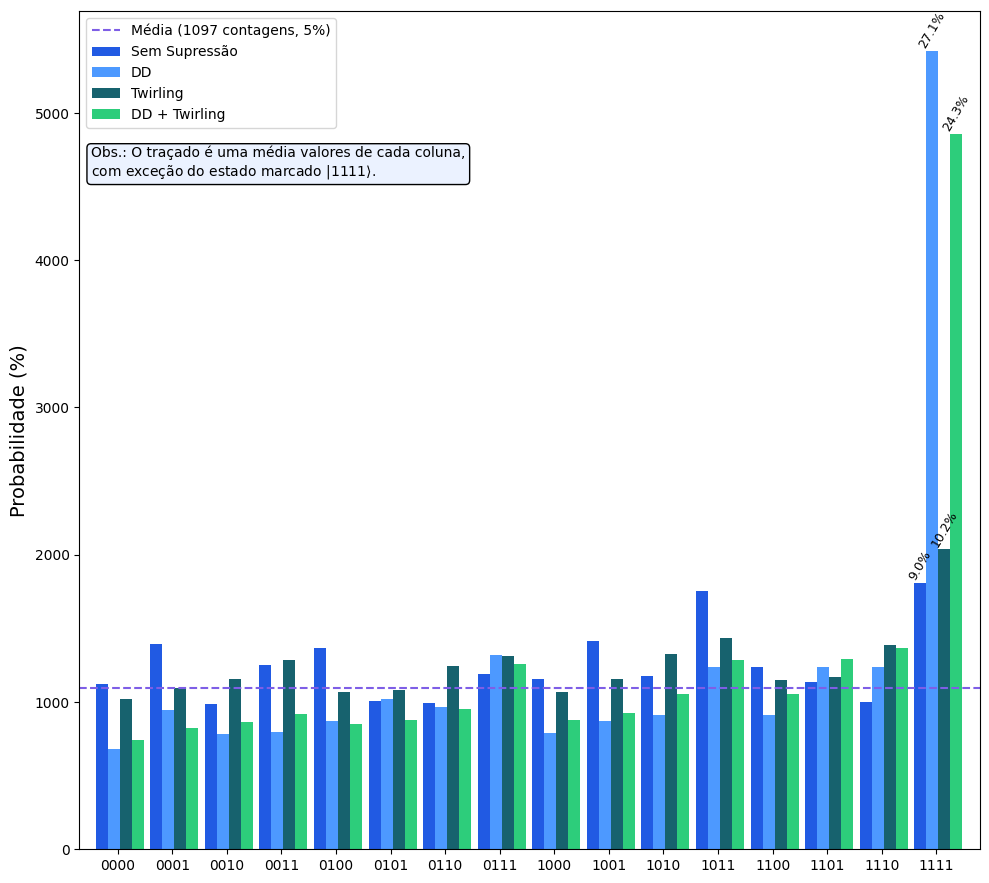
\includegraphics[width=\linewidth]{Imagens/resultBrisbane_3.png}
        \label{subFig: resultBrisbane_3}
    \end{subfigure}
    
    \vspace{0.3em}
    {\small Fonte: do autor} 
\end{figure}

\begin{figure}[ht!]
    \centering
    \captionsetup{justification=centering}
    \caption{Resultados de \textit{ibm\_torino}}
    \label{fig: resultTorino}

    \begin{subfigure}[b]{0.46\textwidth}
        \centering
        \caption{Histograma de \textit{ibm\_torino} com $optim\_lvl = 2$}
        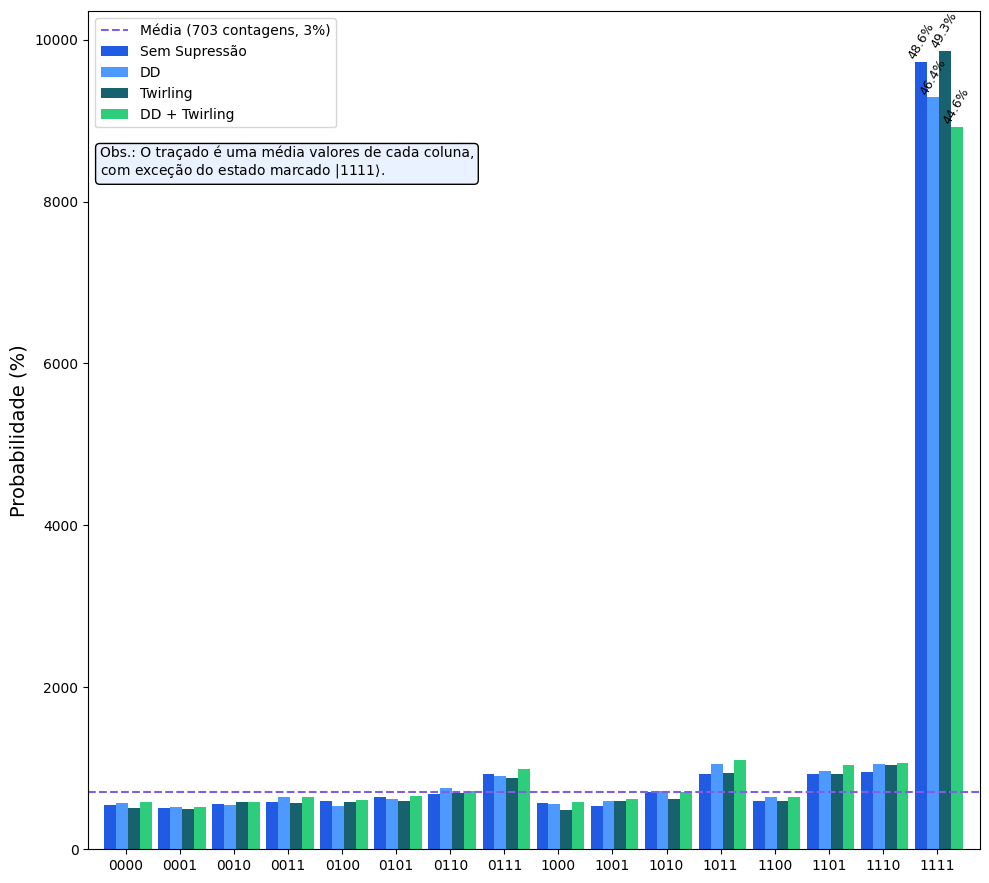
\includegraphics[width=\linewidth]{Imagens/resultTorino_2.png}
        \label{subFig: resultTorino_2}
    \end{subfigure}
    \hspace{1cm}
    \begin{subfigure}[b]{0.46\textwidth}
        \centering
        \caption{Histograma de \textit{ibm\_torino} com $optim\_lvl = 3$}
        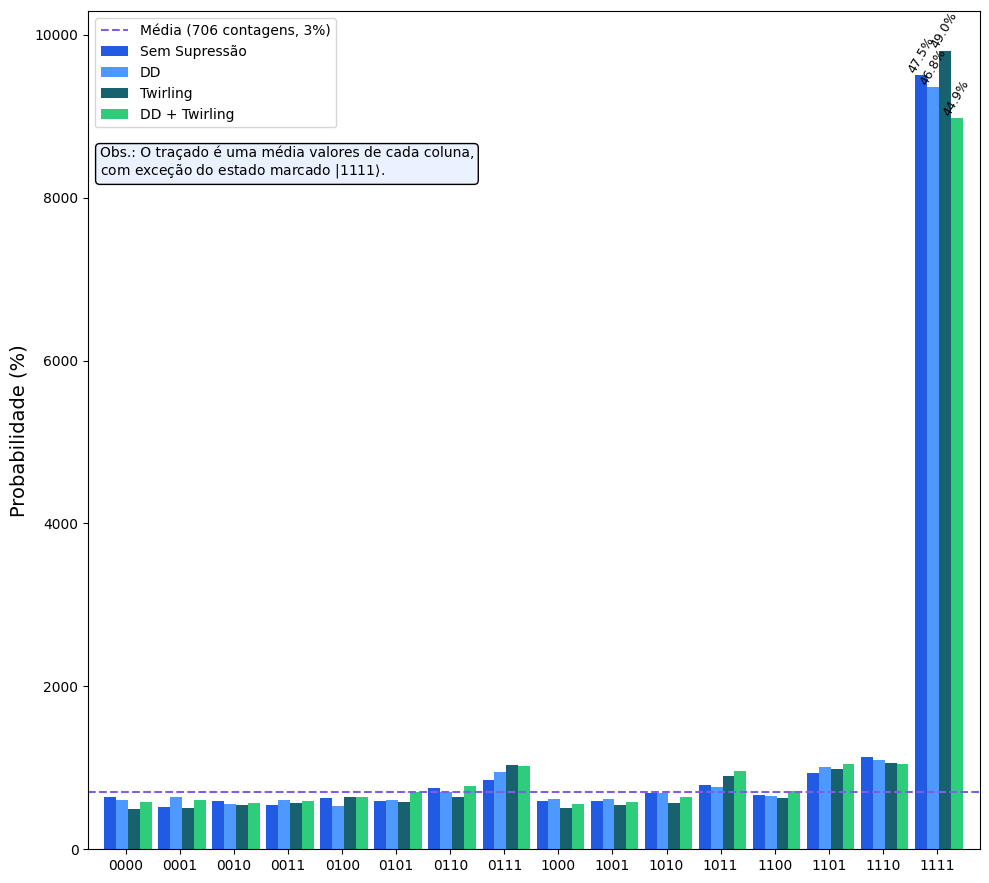
\includegraphics[width=\linewidth]{Imagens/resultTorino_3.png}
        \label{subFig: resultTorino_3}
    \end{subfigure}
    
    \vspace{0.3em}
    {\small Fonte: do autor} 
\end{figure}
% \chapter{ELEMENTOS DO TEXTO}
\label{sec: elementos}

% \begin{simbolo} %patagrafo == 2 tabs
%     \tab\tab$MCZ$
%     \addcontentsline{los}{simbolo}{MCZ \tab Porta Lógica Z-Multi-Controlada}
% \end{simbolo}

Este capítulo apresenta o uso básico de equações, figuras e tabelas no código da monografia, bem como o posicionamento das legendas, segundo as normas da UFLA.

\section{Utilizando Recursos do \LaTeX}

\subsection{Inserindo Comandos Definidos}

Esta subseção apresenta o uso de comandos definidos pelo usuário no pre\^{a}mbulo do arquivo principal \LaTeX e alguns exemplos do modo matemático. Por exemplo, na texto a seguir é utilizado o comando  \verb+\defs+, definido anteriormente pelo próprio autor do texto:

\begin{quote}
Os conjuntos fundamentais da teoria são os \defs{conjuntos elementares}. Se $E$ é um conjunto elementar, $des(E)$ denota a descrição dessa classe de equivalência. Essa descrição é função do conjunto de atributos que define $R$. Note que, dados $x,y \in E$, onde $E$ é um conjunto elementar em $A$, $x$ e $y$ são indiscerníveis, i.e., no espaço $A=(U,R)$ não se consegue distinguir $x$ de $y$, pois $des(x) = des(y) = des(E)$. 
\end{quote}

\subsection{Inserindo Figuras}

A Figura~\ref{fig:exemplo} é apenas um exemplo de figura para que o usuário da classe possa saber como uma figura pode ser inserida e referenciada automaticamente no texto.É importante observar que legendas de figuras ficam abaixo de seu conteúdo.

\begin{figure}[!htb]
\centering
\caption{Uma Figura de Exemplo} %legenda

\includegraphics[scale=0.9]{Imagens/gradpenguin.png}\\  % o 0.9 indica 90% do tamanho original
% pdfLaTeX aceita figuras no formato PNG, JPG ou PDF
% figuras vetoriais podem ser exportadas para eps e depois convertidas para pdf usando epstopdf
{\small Fonte: fonte da figura} %Fonte da imagem
\label{fig:exemplo} %rotulo para refencia
\end{figure}

\subsection{Inserindo Saídas de Comandos e Código}

A menos que sejam trechos pequenos, saídas de comandos, trechos de arquivos de configuração e código de aplicativos devem ser inseridos como figura, como mostrado, respectivamente, na Figura~\ref{fig:exemplocomando}, Figura~\ref{fig:exemploconfig} e Figura~\ref{fig:exemplocodigo1}. Para comandos e configuração, recomenda-se o uso do pacote {\tt fancyvrb}, o que pode ser visto na Figura~\ref{fig:exemplocomando} e Figura~\ref{fig:exemploconfig}.

Para inserção de código, recomenda-se o uso do pacote {\tt listings}, que permite melhor apresentação do mesmo, o que é mostrado na Figura~\ref{fig:exemplocodigo1}. Além disso, esses dois pacotes permitem a inserção de texto/código em arquivos externos, sem inclusão direta no arquivo \LaTeX. Isso pode ser verificado no exemplo de uso do {\tt listings} apresentado na Figura~\ref{fig:exemplocodigo2}

\begin{figure}[!htb]
\centering
\caption{Inserindo Comando} %legenda
\begin{Verbatim}[fontsize=\small]
$ dir monografia*
-rw-r--r--  1 joukim users   3650 Set 12 17:56 monografia.aux
-rw-r--r--  1 joukim users   6366 Set 12 17:43 monografia.bbl
-rw-r--r--  1 joukim users    290 Set 12 17:56 monografia.lof
-rw-r--r--  1 joukim users  27937 Set 12 17:56 monografia.log
-rw-r--r--  1 joukim users    194 Set 12 17:56 monografia.lot
-rw-r--r--  1 joukim users    715 Set 12 17:56 monografia.out
-rw-r--r--  1 joukim users 159243 Set 12 17:56 monografia.pdf
-rw-r--r--  1 joukim users   4559 Set 12 17:47 monografia.tex
-rw-r--r--  1 joukim users    964 Set 12 17:56 monografia.toc
\end{Verbatim} 
%$ - esse comentário é para não confundir editor de texto
{\small Fonte: fonte da figura} %Fonte da imagem
\label{fig:exemplocomando} %rotulo para refencia
\end{figure}

\begin{figure}[!htb]
\centering
\caption{Inserindo Trecho de Arquivo de Configuração} %legenda
\begin{Verbatim}[fontsize=\small]
// named.conf for Red Hat caching-nameserver
options {
        directory "/var/named";
        dump-file "/var/named/data/cache_dump.db";
        statistics-file "/var/named/data/named_stats.txt";
        // query-source address * port 53;
};
\end{Verbatim} 
{\small Fonte: fonte da figura} %Fonte da imagem
\label{fig:exemploconfig} %rotulo para refencia
\end{figure}


\begin{figure}[!htb]
\centering
\caption{Inserindo Código Diretamente no Arquivo \LaTeX} %legenda
\begin{lstlisting}
// exit the program
public void on_buttonExit_clicked() {
	System.exit(0);
}

// copy data
public void on_buttonCopy_clicked() {
	labelShow.setText(entryData.getText());
}

// print version of Java
public static void main(String[] args) {
	System.out.println(System.getProperty("java.fullversion"));
}
\end{lstlisting} 
{\small Fonte: fonte da figura} %Fonte da imagem
\label{fig:exemplocodigo1} %rotulo para refencia
\end{figure}


% \begin{figure}[H]
% \centering
% \caption{Inserindo Código a Partir do Código-Fonte} %legenda
% \label{fig:exemplocodigo2} %rotulo para refencia
% \lstinputlisting{Hello.java}
% {\small Fonte: fonte da figura} %Fonte da imagem
% \end{figure}

\subsection{Inserindo Quadros e Tabelas}

Escrever um quadro ou tabela e referenciá-los é bem simples. Por exemplo, o Quadro~\ref{tab:exemplo} ilustra a criação de um quadro, tendo aqui seu referenciamento no texto. É importante observar o posicionamento da legenda antes do corpo da tabela e da fonte após. Outros exemplos são mostrados na Tabela~\ref{tab:outro} e Tabela~\ref{tab:maisum}.

\begin{quadro}[htb]
  \begin{center}
    \caption{Exemplo de Quadro} 
    \label{tab:exemplo}
    \vspace{0.2cm}
    \footnotesize
    \begin{tabular}{|c|c|c|c|c|c|}
      \hline
      $U$ & $vitA$ & $vitC$ & $vitD$ & $prot$ & $lip$ \\
      \hline
      \hline
      $d_1$ & 1 & 3 & 4 & 2 & 3\\
      $d_2$ & 1 & 3 & 3 & 3 & 2\\
      $d_3$ & 1 & 3 & 4 & 3 & 1\\
      $d_4$ & 3 & 5 & 2 & 5 & 2\\
      $d_5$ & 4 & 5 & 2 & 5 & 1\\
      $d_6$ & 3 & 5 & 2 & 3 & 4\\
      $d_7$ & 4 & 4 & 1 & 3 & 2\\
      \hline 
    \end{tabular}
  \end{center}
  \centering {\small Fonte: fonte do quadro} %Fonte do quadro
\end{quadro}

\begin{table}[!htb]
\begin{center}
  \caption{Recursos do {\ttfamily syslog}}
  \label{tab:outro}
  \small
  \begin{tabular}{l|p{9cm}}
    \hline
    \rowcolor[gray]{.9}
    \bf Recurso & \bf {\em Daemons} Associados (Alguns Exemplos) \\
    \hline
    \hline
    \tt kern & \em kernel  \\
    \tt user & processos dos usuários ({\tt ntpd}) \\
    \tt mail & softwares relacionados com o correio eletrônico ({\tt sendmail})\\
    \tt daemon & {\em daemons} do sistema ({\tt gated}, {\tt inetd}, 
    {\tt named}, {\tt ntpd})\\
    \tt auth &  comandos relacionados à autorização e segurança 
    ({\tt login}, {\tt rlogin}, {\tt su}, {\tt passwd}) \\
    \tt lpr & spool de impressão ({\tt lpd})\\
    \tt news & sistema de notícias da usenet ({\tt nnrpd})\\
    \tt uucp & destinado ao {\tt uucp}\\
    \tt cron & relacionado ao {\em daemon} {\tt cron}\\
    \tt mark &  registros de data/hora gerados a intervalos regulares 
    ({\tt syslogd})\\
    \tt local0-7 & 8 tipos de mensagens locais \newline
    ({\tt tcpd -- local7}, {\tt sudo -- local2}, {\tt popper - local0}) \\
    \tt syslog &  mensagens internas ao {\tt syslog}\\
    \tt authpriv & mensagens privadas de autorização\\
    \tt ftp & associado ao {\tt ftpd} ({\em daemon} do {\tt ftp}) \\
    \tt * &  todos os recursos com exceção do {\tt mark}\\
    \hline
  \end{tabular}
\end{center}
\centering {\small Fonte: fonte da tabela} %Fonte da tabela
\end{table}

\begin{table}[!htb]
\caption{Opções do Comando {\ttfamily at}}
\label{tab:maisum}
\begin{center}
  \small
  \begin{tabular}{l|p{9cm}}
    \hline 
    \rowcolor[gray]{.9}
    \bf Opção & \bf Descrição\\
    \hline
    \hline 
    \tt -c & exibe os jobs registrados\\
    \tt -d & remove um job específico\\
    \tt -f & permite que os comandos sejam lidos a partir de um arquivo (não pela
    entrada-padrão)\\
    \tt -l & lista todos os jobs associados a um usuário\\
    \tt -m & envia um e-mail ao usuário quando o job for finalizado\\
    \hline \end{tabular}\\
\end{center}
\centering {\small Fonte: fonte da tabela} %Fonte da tabela
\end{table}

\subsection{Inserindo Equações}

Equações devem ser numeradas, com a numeração, em parênteses à direita da mesma. Isso é ilustrado na Equação~\ref{eq:exemplo}.

\begin{equation}
\label{eq:exemplo}
f'(x) = \int^{x^2}_{x^{-1}} xdx 
\end{equation}


\section{Usando Referências}
A equipe do curso não impõe normas rígidas para o formato a ser adotado nas referências bibliográficas, desde que seja usado um padrão acadêmico conhecido. Caso os autores não possuam um padrão preferencial, recomenda-se o formato estipulado pela ABNT \cite{NBR6023:2002}. A Biblioteca Central da UFLA disponibiliza um manual \cite{BIBUFLA2001} que orienta o uso dessas normas. Se os autores estiverem utilizando \LaTeX, recomenda-se o uso do pacote Abn\TeX\footnote{Disponível em \url{http://abntex.codigolivre.org.br/}.} \cite{Weber2003}. 

Obviamente, recomenda-se a leitura de textos sobre a escrita acadêmica e produção de trabalhos de conclusão para garantir não só qualidade estética e de formatação, mas também de conteúdo. Entre outros, pode-se recomendar a leitura de \cite{Silva2005}, \cite{Martins2000}, \cite{Gil2002}, \cite{Franca2001}, \cite{Eco1996}, \cite{Moura1998}, \cite{Booth2000}, \cite{Hexsel2004}, \cite{Porto2002} e \cite{Henz2003}. 


\chapter{CONCLUSÃO}
\label{sec: conclusao}



%==============================================================================
% Incluindo bibliografia
%\bibliographystyle{plain}             % estilo para labels em numeros
%\bibliographystyle{alpha}             % estilo para labels em iniciais
\bibliographystyle{abntex2-alf}           % estilo para referências usando ABNT, 
                                       % precisa instalar o abntex para usar!!!

\referencias
\bibliography{referencias}			% arquivo exemplo refbib.bib
%==============================================================================
% Incluindo anexos num1erados com letras maiusculas.
\appendix
\apendice{Demonstração do Circuito}
\label{ap:apendiceA}

Com a finalidade de entender o que acontece em cada parte do circuito + será feita a demonstração passo a passo das operações a cada camada.

Seja $\ket{\psi}$ o estado inicial do espaço formado pelos $4$ qubits + com valor inicial dado por $\ket{\psi} = \ket{0000}$. Aplicaremos portas \textit{Hadamard} em cada qubit como parte da primeira etapa do Algoritmo de Grover: a preparação inicial. Essa operação resulta em:

\begin{enumerate}[nosep,leftmargin=*]
    \item Preparação inicial: aplicação das portas \textit{H}'s (Figura~\ref{fig:psi1}):
    \begin{flalign*}
        H^{\otimes 4}\ket{\psi} &= \ket{\psi_1} = \frac{1}{4} \Bigl(\ket{0000} + \ket{0001} + \ket{0010} + \ket{0011} + \ket{0100} + \ket{0101} + \ket{0110} && \\ &
        + \ket{0111} +  \ket{1000} + \ket{1001} + \ket{1010} + \ket{1011} + \ket{1100} + \ket{1101} + \ket{1110} + \ket{1111}\Bigr) &&
    \end{flalign*}
    \vspace{-30pt}
    \begin{figure}[ht!]
        \centering
        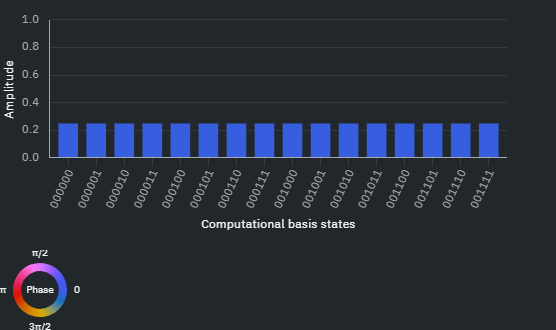
\includegraphics[trim=0mm 47mm 15mm 0mm, clip, width=.6\linewidth]{Imagens/EvPsi/Psi1.png}
        \caption{Aplicação das portas \textit{H}'s na preparação inicial.}
        \label{fig:psi1}
    
    {\small Fonte: IBM-\textit{Quantum Learning / Composer}.}
    \end{figure}
    \item Aplicar o oráculo \(U_f\) que marca o estado \(\ket{1111}\) invertendo seu sinal (Figura~\ref{fig:psi2}):
        \begin{flalign*}
        U_f\ket{\psi_1} &= \ket{\psi_2} = \frac{1}{4} \Bigl(\ket{0000} + \ket{0001} + \ket{0010} + \ket{0011} + \ket{0100} + \ket{0101} + \ket{0110} && \\ & 
        + \ket{0111} + \ket{1000} + \ket{1001} + \ket{1010} + \ket{1011} + \ket{1100} + \ket{1101} + \ket{1110} - \ket{1111}\Bigr) &&
    \end{flalign*}
    \vspace{-30pt}
    \begin{figure}[ht!]
        \centering
        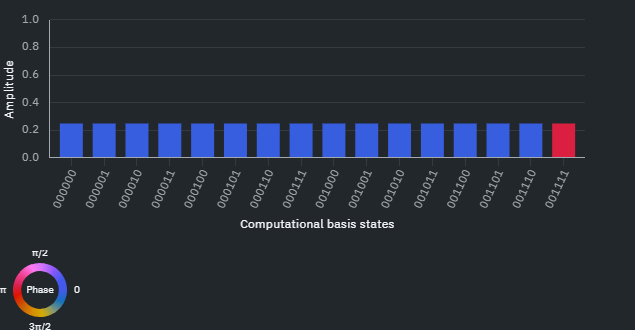
\includegraphics[trim=0mm 47mm 15mm 0mm, clip, width=.6\linewidth]{Imagens/EvPsi/Psi2.png}
        \caption{Aplicação do oráculo \(U_f\), que inverte o sinal do estado \(\ket{1111}\).}
        \label{fig:psi2}
    
    {\small Fonte: IBM-\textit{Quantum Learning / Composer}.}
    \end{figure}

    \item Início da operação de difusão: aplicar portas \textit{Hadamard} (Figura~\ref{fig:psi3}):
        \begin{flalign*}
        H^{\otimes 4}\ket{\psi_2} &= \ket{\psi_3} = \frac{1}{8} \Bigl( 7\ket{0000} + \ket{0001} + \ket{0010} - \ket{0011} + \ket{0100} - \ket{0101} - \ket{0110} && \\ & 
        + \ket{0111} + \ket{1000} - \ket{1001} - \ket{1010} + \ket{1011} - \ket{1100} + \ket{1101} + \ket{1110} - \ket{1111} \Bigr) &&
    \end{flalign*}
    \vspace{-30pt}
    \begin{figure}[ht!]
        \centering
        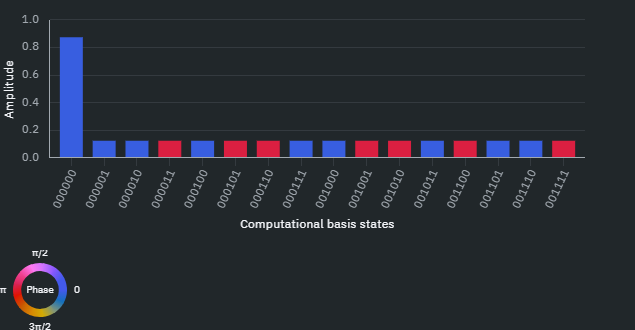
\includegraphics[trim=0mm 47mm 15mm 0mm, clip, width=.6\linewidth]{Imagens/EvPsi/Psi3.png}
        \caption{Aplicação das portas \textit{Hadamard} no início da operação de difusão.}
        \label{fig:psi3}
    
    {\small Fonte: IBM-\textit{Quantum Learning / Composer}.}
    \end{figure}

    \item Aplicar portas \(X\) (Figura~\ref{fig:psi4}):
  \begin{flalign*}
        X^{\otimes 4}\ket{\psi_3} &= \ket{\psi_4} = \frac{1}{8} \Bigl( 7\ket{1111} + \ket{1110} + \ket{1101} - \ket{1100} + \ket{1011} - \ket{1010} - \ket{1001} + \ket{1000} && \\ &
        + \ket{0111} - \ket{0110} - \ket{0101} + \ket{0100} - \ket{0011} + \ket{0010} + \ket{0001} - \ket{0000}\Bigr) && \\[6pt]
        &= \frac{1}{8} \Bigl(-\ket{0000} + \ket{0001} + \ket{0010} - \ket{0011} + \ket{0100} - \ket{0101} - \ket{0110} + \ket{0111} && \\ &
        + \ket{1000} - \ket{1001} - \ket{1010} + \ket{1011} - \ket{1100} + \ket{1101} + \ket{1110} + 7\ket{1111}\Bigr) &&
    \end{flalign*}
    \vspace{-30pt}
    \begin{figure}[ht!]
        \centering
        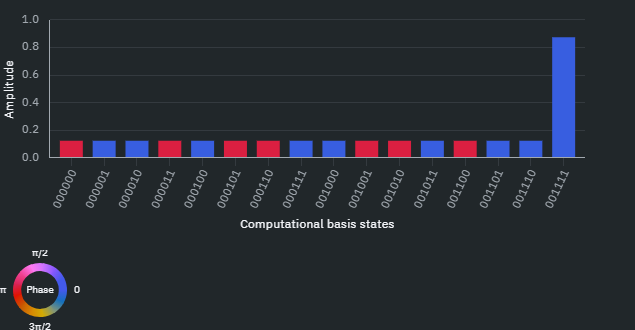
\includegraphics[trim=0mm 47mm 15mm 0mm, clip, width=.6\linewidth]{Imagens/EvPsi/Psi4.png}
        \caption{Aplicação das portas $X$ no operador de difusão.}
        \label{fig:psi4}
    
    {\small Fonte: IBM-\textit{Quantum Learning / Composer}.}
    \end{figure}

    \item Aplicar a porta $MCZ$ (Figura~\ref{fig:psi5}):
        \begin{flalign*}
        MCZ \ket{\psi_4} &= \ket{\psi_5} = \frac{1}{8} \Bigl(-\ket{0000} + \ket{0001} + \ket{0010} - \ket{0011} + \ket{0100} - \ket{0101} - \ket{0110} && \\ 
        + \ket{0111} & + \ket{1000} - \ket{1001} - \ket{1010} + \ket{1011} - \ket{1100} + \ket{1101} + \ket{1110} - 7 \ket{1111}\Bigr) &&
    \end{flalign*}
    \vspace{-30pt}
    \begin{figure}[ht!]
        \centering
        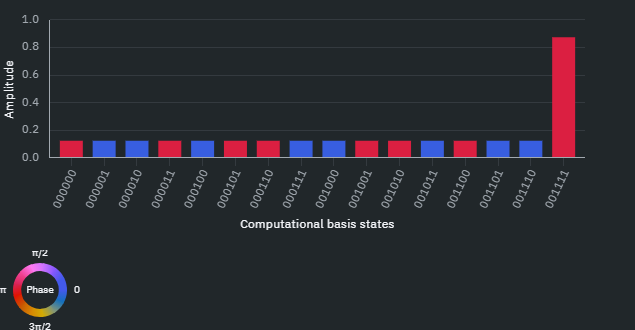
\includegraphics[trim=0mm 47mm 15mm 0mm, clip, width=.6\linewidth]{Imagens/EvPsi/Psi5.png}
        \caption{Aplicação da porta $MCZ$ no operador de difusão.}
        \label{fig:psi5}
    
    {\small Fonte: IBM-\textit{Quantum Learning / Composer}.}
    \end{figure}
    \item Aplicar portas $X$ novamente (Figura~\ref{fig:psi6}):
   \begin{flalign*}
        X^{\otimes 4} \ket{\psi_5} &= \ket{\psi_6} = \frac{1}{8} \Bigl( -\ket{1111} + \ket{1110} + \ket{1101} - \ket{1100} + \ket{1011} - \ket{1010} - \ket{1001}  && \\
        + \ket{1000} & + \ket{0111} - \ket{0110} - \ket{0101} + \ket{0100} - \ket{0011} + \ket{0010} + \ket{0001} - 7 \ket{0000}\Bigr) && \\[6pt]
        &= \frac{1}{8} \Bigl(-7 \ket{0000} + \ket{0001} + \ket{0010} - \ket{0011} + \ket{0100} - \ket{0101} - \ket{0110} + \ket{0111} && \\ & 
        + \ket{1000} - \ket{1001} - \ket{1010} + \ket{1011} - \ket{1100} + \ket{1101} + \ket{1110} - \ket{1111} \Bigr) &&
    \end{flalign*}
    \vspace{-30pt}
    \begin{figure}[ht!]
        \centering
        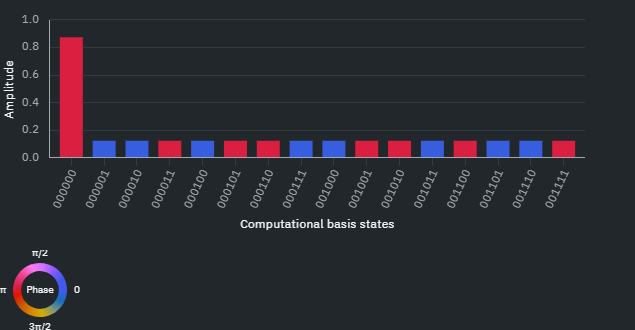
\includegraphics[trim=0mm 47mm 15mm 0mm, clip, width=.6\linewidth]{Imagens/EvPsi/Psi6.png}
        \caption{Segunda aplicação das portas $X$ no operador de difusão.}
        \label{fig:psi6}
    
    {\small Fonte: IBM-\textit{Quantum Learning / Composer}.}
    \end{figure}

    \item Aplicar portas \textit{Hadamard} novamente (Figura~\ref{fig:psi7}):
\begin{flalign*}
    H^{\otimes 4} \ket{\psi_6} &= \ket{\psi_7} = \frac{1}{16} \Bigl( 
        -3\ket{0000} - 3\ket{0001} - 3\ket{0010} - 3\ket{0011} - 3\ket{0100} - 3\ket{0101} && \\ &\quad - 3\ket{0110} - 3\ket{0111} - 3\ket{1000} - 3\ket{1001} - 3\ket{1010} && \\
        & - 3\ket{1011} - 3\ket{1100} - 3\ket{1101} - 3\ket{1110} - 11\ket{1111} 
    \Bigr) && \\[6pt]
    &= -\frac{3}{16} \Bigl(
        \ket{0000} + \ket{0001} + \ket{0010} + \ket{0011} + \ket{0100} + \ket{0101} + \ket{0110} + \ket{0111} && \\
        & + \ket{1000} + \ket{1001} + \ket{1010} + \ket{1011} + \ket{1100} + \ket{1101} + \ket{1110} + \frac{11}{3} \ket{1111}
    \Bigr) &&
\end{flalign*}
    \vspace{-30pt}
    \begin{figure}[ht!]
        \centering
        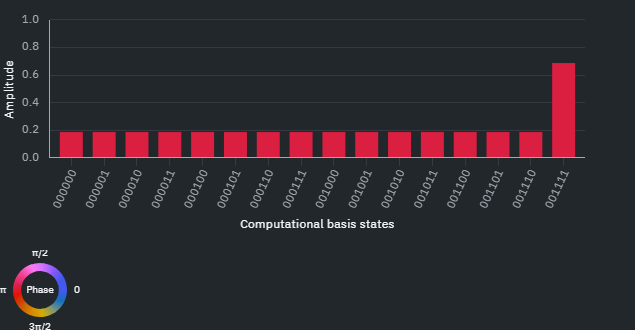
\includegraphics[trim=0mm 47mm 15mm 0mm, clip, width=.6\linewidth]{Imagens/EvPsi/Psi7.png}
        \caption{Aplicação final das portas \textit{Hadamard} na primeira iteração.}
        \label{fig:psi7}
    
    {\small Fonte: IBM-\textit{Quantum Learning / Composer}.}
    \end{figure}

    O sétimo passo finaliza a primeira iteração, mas precisamos repetir o processo mais duas vezes.

    \item Marcar novamente o estado buscado pelo oráculo \(U_f\) (Figura~\ref{fig:psi8}):
    \begin{flalign*}
        U_f \ket{\psi_7} &= \ket{\psi_8} = -\frac{3}{16} \Bigl( \ket{0000} + \ket{0001} + \ket{0010} + \ket{0011} + \ket{0100} + \ket{0101} + \ket{0110} && \\  
         + \ket{0111} &+ \ket{1000} + \ket{1001} + \ket{1010} + \ket{1011} + \ket{1100} + \ket{1101} + \ket{1110} - \frac{11}{3} \ket{1111} \Bigr)
    \end{flalign*}
    \vspace{-30pt}
    \begin{figure}[ht!]
        \centering
        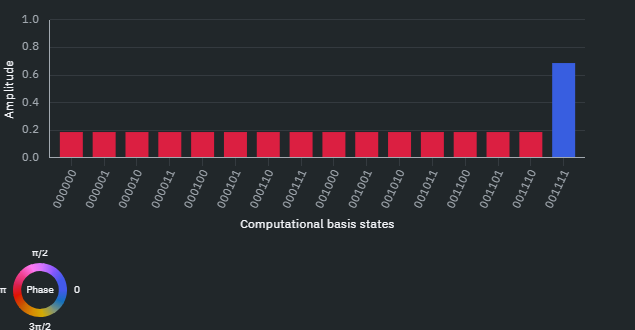
\includegraphics[trim=0mm 47mm 15mm 0mm, clip, width=.6\linewidth]{Imagens/EvPsi/Psi8.png}
        \caption{Aplicação do oráculo \(U_f\) na segunda iteração.}
        \label{fig:psi8}
    
    {\small Fonte: IBM-\textit{Quantum Learning / Composer}.}
    \end{figure}

    Após o oráculo, devemos aplicar o operador de difusão.

    \item Aplicar portas \textit{Hadamard} (Figura~\ref{fig:psi9}):
    \begin{flalign*}
        H^{\otimes 4} \ket{\psi_8} &= \ket{\psi_9} = \frac{7}{32} \Bigl(-\frac{17}{7} \ket{0000} - \ket{0001} - \ket{0010} + \ket{0011} - \ket{0100} + \ket{0101} + \ket{0110} && \\\ &
        - \ket{0111} - \ket{1000} + \ket{1001} + \ket{1010} - \ket{1011} + \ket{1100} - \ket{1101} - \ket{1110} + \ket{1111} \Bigr)
    \end{flalign*}
    \vspace{-30pt}
    \begin{figure}[ht!]
        \centering
        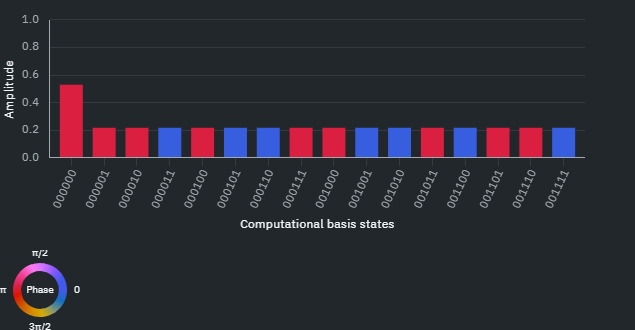
\includegraphics[trim=0mm 47mm 15mm 0mm, clip, width=.6\linewidth]{Imagens/EvPsi/Psi9.png}
        \caption{Aplicação das portas \textit{Hadamard} na operação de difusão da segunda iteração.}
        \label{fig:psi9}
    
    {\small Fonte: IBM-\textit{Quantum Learning / Composer}.}
    \end{figure}

    \item Aplicar portas $X$ (Figura~\ref{fig:psi10}):
    \begin{flalign*}
        X^{\otimes 4} \ket{\psi_9} &= \ket{\psi_{10}} = \frac{7}{32} \Bigl(-\frac{17}{7} \ket{1111} - \ket{1110} - \ket{1101} + \ket{1100} - \ket{1011} + \ket{1010} + \ket{1001} && \\ & - \ket{1000} - \ket{0111} + \ket{0110} + \ket{0101} - \ket{0100} + \ket{0011} - \ket{0010} - \ket{0001} + \ket{0000} \Bigr) && \\[6pt] 
        &= \frac{7}{32} \Bigl( \ket{0000} - \ket{0001} - \ket{0010} + \ket{0011} - \ket{0100} + \ket{0101} + \ket{0110} - \ket{0111} && \\ & - \ket{1000} + \ket{1001} + \ket{1010} - \ket{1011} + \ket{1100} - \ket{1101} - \ket{1110} - \frac{17}{7} \ket{1111} \Bigr)
    \end{flalign*}
    \vspace{-30pt}
    \begin{figure}[ht!]
        \centering
        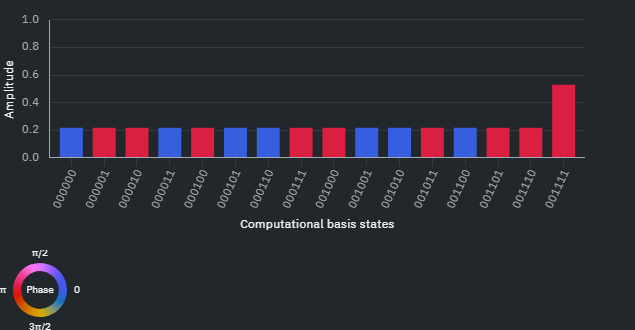
\includegraphics[trim=0mm 47mm 15mm 0mm, clip, width=.6\linewidth]{Imagens/EvPsi/Psi10.png}
        \caption{Aplicação das portas $X$ no operador de difusão da segunda iteração.}
        \label{fig:psi10}
    
    {\small Fonte: IBM-\textit{Quantum Learning / Composer}.}
    \end{figure}

    \item Aplicar porta $MCZ$ (Figura~\ref{fig:psi11}):
    \begin{flalign*}
        MCZ \ket{\psi_{10}} &= \ket{\psi_{11}} = \frac{7}{32} \Bigl( \ket{0000} - \ket{0001} - \ket{0010} + \ket{0011} - \ket{0100} + \ket{0101} + \ket{0110} && \\ 
        - \ket{0111} & - \ket{1000} + \ket{1001} + \ket{1010} - \ket{1011} + \ket{1100} - \ket{1101} - \ket{1110} + \frac{17}{7} \ket{1111} \Bigr)
    \end{flalign*}
    \vspace{-30pt}
    \begin{figure}[ht!]
        \centering
        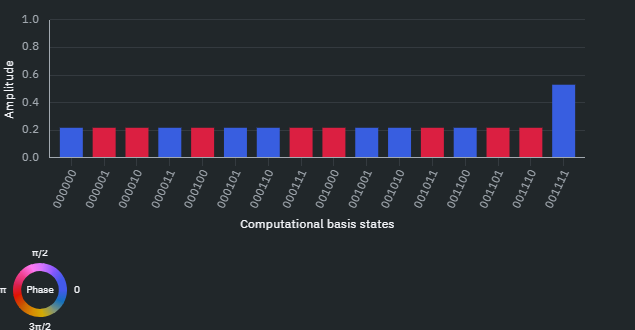
\includegraphics[trim=0mm 47mm 15mm 0mm, clip, width=.6\linewidth]{Imagens/EvPsi/Psi11.png}
        \caption{Aplicação da porta $MCZ$ na segunda iteração do operador de difusão.}
        \label{fig:psi11}
    
    {\small Fonte: IBM-\textit{Quantum Learning / Composer}.}
    \end{figure}

    \item Aplicar portas $X$ novamente (Figura~\ref{fig:psi12}):
    \begin{flalign*}
        X^{\otimes 4} \ket{\psi_{11}} &= \ket{\psi_{12}} = \frac{7}{32} \Bigl( \ket{1111} - \ket{1110} - \ket{1101} + \ket{1100} - \ket{1011} + \ket{1010} + \ket{1001} && \\ - \ket{1000} & - \ket{0111} + \ket{0110} + \ket{0101} - \ket{0100} + \ket{0011} - \ket{0010} - \ket{0001} + \frac{17}{7} \ket{0000} \Bigr) && \\[6pt]
        &= \frac{7}{32} \Bigl( \frac{17}{7} \ket{0000} - \ket{0001} - \ket{0010} + \ket{0011} - \ket{0100} + \ket{0101} + \ket{0110} - \ket{0111}  && \\ & - \ket{1000} + \ket{1001} + \ket{1010} - \ket{1011} + \ket{1100} - \ket{1101} - \ket{1110} + \ket{1111} \Bigr)
    \end{flalign*}
    \vspace{-30pt}
    \begin{figure}[ht!]
        \centering
        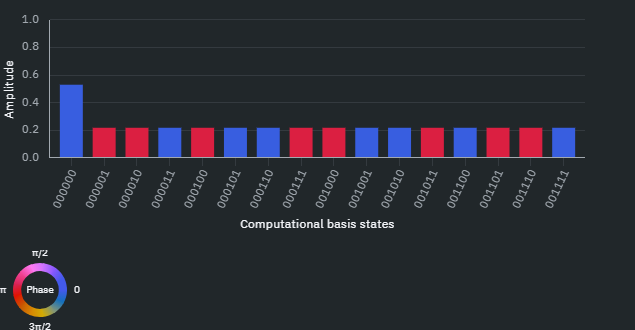
\includegraphics[trim=0mm 47mm 15mm 0mm, clip, width=.6\linewidth]{Imagens/EvPsi/Psi12.png}
        \caption{Segunda aplicação das portas $X$ na segunda iteração do operador de difusão.}
        \label{fig:psi12}
   
    {\small Fonte: IBM-\textit{Quantum Learning / Composer}.}
    \end{figure}

\item Para finalizar a segunda iteração, aplicamos novamente as portas \textit{Hadamard}:
    \begin{flalign*}
        H^{\otimes 4}\ket{\psi_{12}} &= \ket{\psi_{13}} = \frac{5}{64} \Bigl(\ket{0000}+ \ket{0001}+ \ket{0010} + \ket{0011} + \ket{0100} + \ket{0101} + \ket{0110} && \\ + \ket{0111} & + \ket{1000} + \ket{1001} + \ket{1010} + \ket{1011} + \ket{1100} + \ket{1101} + \ket{1110} + \frac{61}{5}\ket{1111}\Bigr)
    \end{flalign*}
    \vspace{-30pt}
    \begin{figure}[ht!]
        \centering
        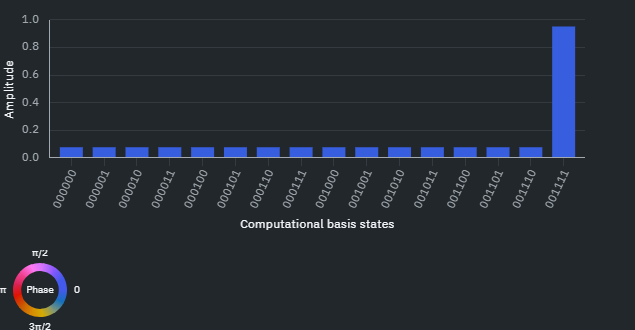
\includegraphics[trim=0mm 47mm 15mm 0mm, clip, width=.6\linewidth]{Imagens/EvPsi/Psi13.png}
        \caption{Aplicação final das portas \textit{Hadamard} na segunda iteração.}
        \label{fig:psi13}
    
    {\small Fonte: IBM-\textit{Quantum Learning / Composer}.}
    \end{figure}

O décimo terceiro passo finaliza a segunda iteração, mas é necessário repetir o processo mais uma vez.

    \item Aplicar o oráculo \(U_f\) mais uma vez (Figura~\ref{fig:psi14}):
    \begin{flalign*}
        U_f\ket{\psi_{13}} &= \ket{\psi_{14}} = \frac{5}{64} (\ket{0000} + \ket{0001} + \ket{0010} + \ket{0011} + \ket{0100} + \ket{0101} + \ket{0110} && \\ + \ket{0111}
        &+ \ket{1000} + \ket{1001} + \ket{1010} + \ket{1011} + \ket{1100} + \ket{1101} + \ket{1110} - \frac{61}{5}\ket{1111}))   
        \end{flalign*}
    \vspace{-30pt}
    \begin{figure}[ht!]
        \centering
        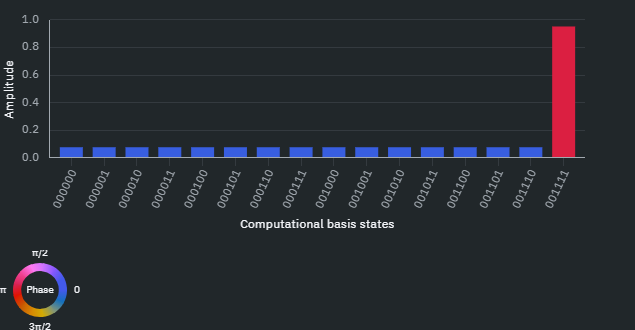
\includegraphics[trim=0mm 47mm 15mm 0mm, clip, width=.6\linewidth]{Imagens/EvPsi/Psi14.png}
        \caption{Aplicação do oráculo \(U_f\) na terceira iteração.}
        \label{fig:psi14}
    
    {\small Fonte: IBM-\textit{Quantum Learning / Composer}.}
    \end{figure}

    \item Aplicar portas \textit{Hadamard} (Figura~\ref{fig:psi15}):
    \begin{flalign*}
  H^{\otimes 4}\ket{\psi_{14}} &= \ket{\psi_{15}} = \frac{33}{128} \Bigl(\frac{7}{33}\ket{0000} + \ket{0001} + \ket{0010} -\ket{0011} + \ket{0100} - \ket{0101} -\ket{0110} && \\ 
  + \ket{0111} & + \ket{1000} -\ket{1001} -\ket{1010} + \ket{1011} - \ket{1100} + \ket{1101} + \ket{1110} - \ket{1111}\Bigr)
        \end{flalign*}
    \vspace{-30pt}
    \begin{figure}[ht!]
        \centering
        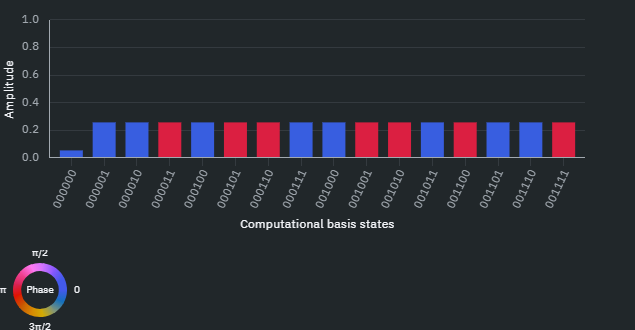
\includegraphics[trim=0mm 47mm 15mm 0mm, clip, width=.6\linewidth]{Imagens/EvPsi/Psi15.png}
        \caption{Aplicação das portas \textit{Hadamard} na operação de difusão da terceira iteração.}
        \label{fig:psi15}
    
    {\small Fonte: IBM-\textit{Quantum Learning / Composer}.}
    \end{figure}

    \item Aplicar portas $X$ (Figura~\ref{fig:psi16}):
    \begin{flalign*}
        X^{\otimes 3}\ket{\psi_{15}} &= \ket{\psi_{16}} = \frac{33}{128} \Bigl(\frac{7}{33}\ket{1111} + \ket{1110} + \ket{1101} - \ket{1100} + \ket{1011} - \ket{1010} -\ket{1001} && \\ & 
        + \ket{1000} + \ket{0111} -\ket{0110} -\ket{0101} - \ket{0100} - \ket{0011} + \ket{0010} + \ket{0001} - \ket{0000}) 
        && \\
        &= \frac{33}{128} (-\ket{0000} + \ket{0001} + \ket{0010} -\ket{0011} + \ket{0100} - \ket{0101} - \ket{0110} + \ket{0111} 
        && \\ &
        + \ket{1000} -\ket{1001} -\ket{1010} + \ket{1011} - \ket{1100} + \ket{1101} + \ket{1110} + \frac{7}{33}\ket{1111})
    \end{flalign*}
    \vspace{-30pt}
    \begin{figure}[ht!]
        \centering
        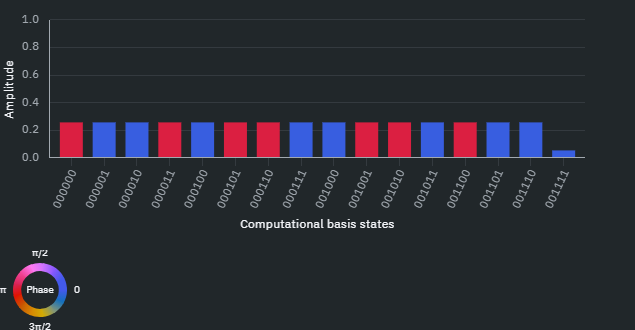
\includegraphics[trim=0mm 47mm 15mm 0mm, clip, width=.6\linewidth]{Imagens/EvPsi/Psi16.png}
        \caption{Aplicação das portas $X$ no operador de difusão da terceira iteração.}
        \label{fig:psi16}
    
    {\small Fonte: IBM-\textit{Quantum Learning / Composer}.}
    \end{figure}

    \item Aplicar porta $MCZ$ (Figura~\ref{fig:psi17}):
    \begin{flalign*}
     MCZ\ket{\psi_{16}} = \ket{\psi_{17}} = \frac{33}{128} \Bigl(&-\ket{0000} + \ket{0001} + \ket{0010} - \ket{0011} + \ket{0100} - \ket{0101} 
     && \\ &
     - \ket{0110} + \ket{0111} + \ket{1000} - \ket{1001} - \ket{1010} 
     && \\ &
     + \ket{1011} - \ket{1100} + \ket{1101} + \ket{1110} - \frac{7}{33}\ket{1111}\Bigr)    
        \end{flalign*}
    \vspace{-30pt}
    \begin{figure}[ht!]
        \centering
        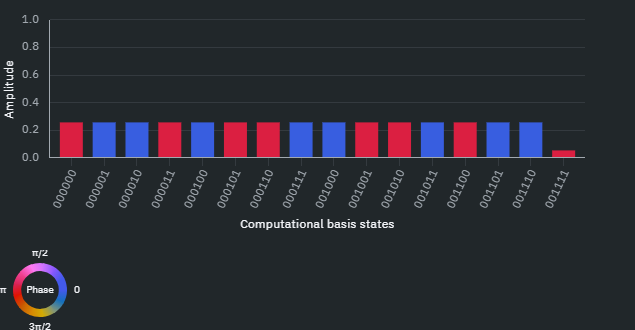
\includegraphics[trim=0mm 47mm 15mm 0mm, clip , width=.6\linewidth]{Imagens/EvPsi/Psi17.png}
        \caption{Aplicação da porta $MCZ$ na terceira iteração do operador de difusão.}
        \label{fig:psi17}
    
    {\small Fonte: IBM-\textit{Quantum Learning / Composer}.}
    \end{figure}

    \item Aplicar portas $X$ (Figura~\ref{fig:psi18}):
    \begin{flalign*}
         X^{4}\ket{\psi_{17}} = \ket{\psi_{18}} = \frac{33}{128} \Bigl(&-\ket{1111}  + \ket{1110}  + \ket{1101} - \ket{1100}  + \ket{1011} 
         && \\ &
         - \ket{1010} - \ket{1001}  + \ket{1000}  + \ket{0111} - \ket{0110} - \ket{0101}  && \\ & + \ket{0100} - \ket{0011}  + \ket{0010}  + \ket{0001} - \frac{7}{33}\ket{0000}\Bigr) 
         && \\
         = \frac{33}{128} \Bigl(&-\frac{7}{33}\ket{0000}  + \ket{0001}  + \ket{0010} - \ket{0011}  && \\ & 
         + \ket{0100} - \ket{0101} - \ket{0110}  + \ket{0111}  + \ket{1000} - \ket{1001} && \\ &
         - \ket{1010}  + \ket{1011} - \ket{1100}  + \ket{1101}  + \ket{1110} - \ket{1111}\Bigr)
    \end{flalign*}
    \vspace{-30pt}
    \begin{figure}[ht!]
        \centering
        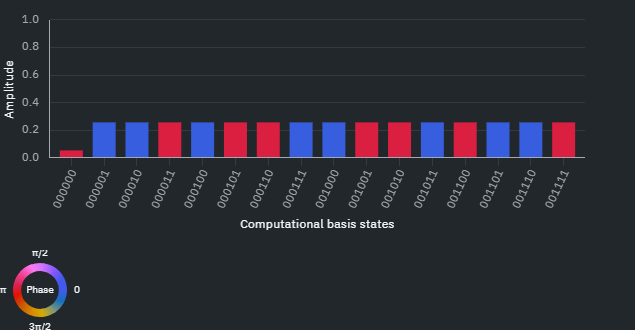
\includegraphics[trim=0mm 47mm 15mm 0mm, clip, width=.6\linewidth]{Imagens/EvPsi/Psi18.png}
        \caption{Última aplicação das portas $X$ na terceira iteração do operador de difusão.}
        \label{fig:psi18}

    {\small Fonte: IBM-\textit{Quantum Learning / Composer}.}
    \end{figure}

        \item Para finalizar a terceira e última iteração, aplicamos novamente as portas \textit{Hadamard} (Figura~\ref{fig:psi19}):
    \begin{flalign*}
         H^{\otimes 4}\ket{\psi_{19}} = \ket{\psi_{20}} = \frac{13}{256} \Bigl(&\ket{0000} + \ket{0001} + \ket{0010} + \ket{0011} + \ket{0100} + \ket{0101} && \\ & 
         + \ket{0110} + \ket{0111} + \ket{1000} + \ket{1001} + \ket{1010} + \ket{1011} && \\ &
         + \ket{1100} + \ket{1101} + \ket{1110} - \frac{251}{13}\ket{1111}\Bigr) 
        \end{flalign*}
    \vspace{-30pt}
    \begin{figure}[ht!]
        \centering
        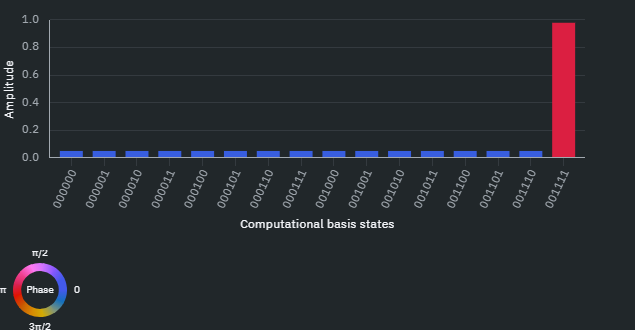
\includegraphics[trim=0mm 47mm 15mm 0mm, clip, width=.6\linewidth]{Imagens/EvPsi/Psi19.png}
        \caption{Probabilidades finais de \(\ket{\psi}\) após as três iterações do Algoritmo de Grover.}
        \label{fig:psi19}

    {\small Fonte: IBM-\textit{Quantum Learning / Composer}.}
    \end{figure}

\end{enumerate}

Ao final do processo, o estado marcado \(\ket{1111}\) aparece com amplitude máxima, o que confirma a eficiência do Algoritmo de Grover em aumentar a probabilidade do estado desejado em um espaço de busca não estruturado.

\vspace{-5pt}
\begin{figure}[ht!]
    \centering
    \captionsetup{justification=centering}    
    \caption{Amplitude e probabilidades após medição final do circuito.}
    \label{fig:AmpProbFinalComposer}
    
    \begin{subfigure}{.48\textwidth}
        \centering
        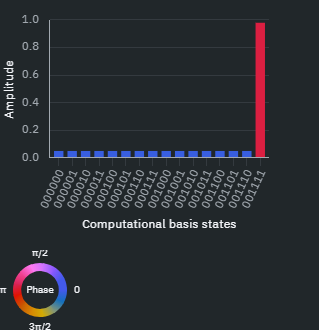
\includegraphics[trim=0mm 47mm 15mm 0mm,clip,width=.7\textwidth]{Imagens/EvPsi/amplitudeFinal.png}
        \subcaption{Amplitude do estado \(\ket{1111}\) igual a $0,98$.}
        \label{subfig:AmpFinalComposer}
    \end{subfigure}
    \begin{subfigure}{.48\textwidth}
        \centering
        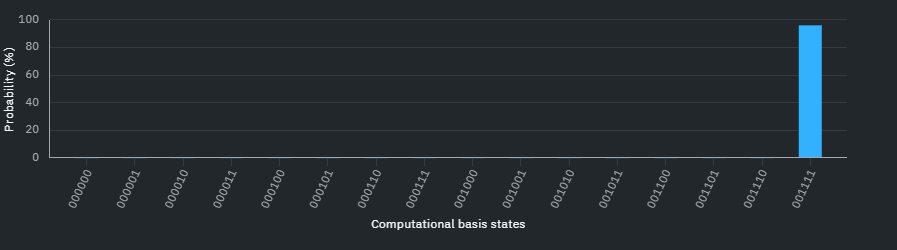
\includegraphics[trim=0mm 0mm 17mm 0mm,clip,width=\textwidth]{Imagens/EvPsi/ProbFinal.png}
        \subcaption{Probabilidades finais de cada estado do espaço de busca, com \(96{,}13\%\) para o estado \(\ket{1111}\).}
        \label{subfig:ProbFinalComposer}
    \end{subfigure}
    
    {\small Fonte: IBM-\textit{Quantum Learning / Composer}.}
\end{figure}

\apendice{Reconstrução de Probabilidades Multi-Qubit a partir do \texttt{Estimator}}
\label{ap:apendiceB}

Ao utilizar o \texttt{Estimator} do \textit{Qiskit}, o resultado retornado consiste nos valores esperados dos operadores de medição, tipicamente expressos em termos de combinações de observáveis do tipo $Z_i$, onde $Z$ é o operador de Pauli-$Z$. 

Para um sistema de $n$ \textit{qubits}, a base computacional $\{\ket{0}, \ket{1}\}$ é associada aos autovalores $+1$ e $-1$ do operador $Z$, respectivamente. Assim, a probabilidade de cada estado base pode ser reconstruída a partir das médias dos produtos de operadores $Z$.

Para o caso de $n=4$, é necessário obter:
\begin{itemize}
    \item As expectativas de 1 ponto: $\langle Z_0 \rangle, ~\langle Z_1 \rangle,~ \langle Z_2 \rangle,~ \langle Z_3 \rangle$.
    \item As expectativas de 2 pontos: $\langle Z_0 Z_1 \rangle,~ \langle Z_0 Z_2 \rangle,~ \dots$.
    \item As expectativas de 3 pontos: $\langle Z_0 Z_1 Z_2 \rangle,~ \dots$.
    \item A expectativa de 4 pontos: $\langle Z_0 Z_1 Z_2 Z_3 \rangle$.
\end{itemize}

A fórmula geral para reconstruir a probabilidade $P(b_0 b_1 b_2 b_3)$, onde $b_k \in \{0,1\}$, é:
\begin{equation}
P(b_0 b_1 b_2 b_3) = \frac{1}{16} \sum_{s_0=0}^1 \sum_{s_1=0}^1 \sum_{s_2=0}^1 \sum_{s_3=0}^1 
\left[ \prod_{j=0}^3 (-1)^{b_j s_j} \right] \langle Z_0^{s_0} Z_1^{s_1} Z_2^{s_2} Z_3^{s_3} \rangle
\end{equation}
onde $Z_j^0 = I$ (identidade no \textit{qubit} $j$) e $Z_j^1 = Z_j$.

Este método é uma aplicação direta da transformada inversa de Walsh–Hadamard sobre as expectativas, convertendo-as em probabilidades na base computacional.

\apendice{Demonstração da Porta \textit{MCZ} a partir de \textit{MCX} e \textit{Hadamard}}
\label{ap:apendiceC}

O objetivo deste apêndice é demonstrar que a porta Z-multi-controlada ($MCZ$) pode ser construída a partir de uma porta X-multi-controlada ($MCX$) e duas portas \textit{Hadamard} (\(H\)). A sequência é dada por:

\begin{equation}
    MCZ = H~\text{MCX}~H
    \label{eq:MCZ}
\end{equation}

onde \(H\) é a porta Hadamard aplicada no qubit alvo da $MCX$.

\subsection*{Demonstração}

A porta $MCZ$ que intenta-se criar possui alvo no último \textit{qubit} apenas, sendo assim, a aplicação das $H$'s deve acontecer somente no último canal. Em termos de portas lógicas e matrizes, isso implica que a Equação~\ref{eq:MCZ}, na verdade, é

\begin{equation}
    MCZ_{16x16} = (I \otimes I \otimes I \otimes H)~MCX_{16x16}~(I \otimes I \otimes I \otimes H)
    \label{eq:MCZ 2}
\end{equation}

A matriz resultante da operação $(I \otimes I \otimes I \otimes H)$ é

\begin{equation}
    \bigl(~I^{\otimes 3}~ \otimes ~H~\bigr)_{16x16} = \frac{1}{\sqrt{2}}
    \begin{bmatrix}
        1 & 1 & 0 & 0 & \cdots & 0 & 0 \\
        1 & -1 & 0 & 0 & \cdots & 0 & 0 \\
        0 & 0 & 1 & 1 & \cdots & 0 & 0 \\
        0 & 0 & 1 & -1 & \cdots & 0 & 0 \\
        \vdots & \vdots & \vdots & \vdots & \ddots & 0 & 0 \\
        0 & 0 & 0 & 0 & 0 & 1 & 1 \\
        0 & 0 & 0 & 0 & 0 & 1 & -1 \\
    \end{bmatrix}
    _{16x16}
\end{equation}

Já a matriz de $MCX$ é

\begin{equation}
    MCX_{16x16} =
    \begin{bmatrix}
        1 & 0 & \cdots & 0 & 0 \\
        0 & 1 & \cdots & 0 & 0 \\
        \vdots & \vdots & \ddots & 0 & 0 \\
        0 & 0 & 0 & 0 & 1 \\
        0 & 0 & 0 & 1 & 0 
    \end{bmatrix}
    _{16x16}
\end{equation}

Voltando à Equação~\ref{eq:MCZ 2}, precisamos fazer o produto
As matrizes correspondentes a $X$, $Z$ e $H$ são, respectivamente

Para um sistema com múltiplos qubits, considere uma MCX com \(n-1\) qubits de controle e 1 qubit alvo:

\begin{equation}
    \text{MCX}\ket{c_1 c_2 \dots c_{n-1} t} = \ket{c_1 c_2 \dots c_{n-1}} \otimes X^{c_1 \cdots c_{n-1}}\ket{t}
\end{equation}

Aplicando Hadamard antes e depois da MCX no qubit alvo:

\begin{align*}
    H \cdot MCX \cdot H \ket{c_1 c_2 \dots c_{n-1} t} 
    &= H \cdot MCX \bigl( \ket{c_1 c_2 \dots c_{n-1}} \otimes H\ket{t} \bigr) \\
    &= H \bigl( \ket{c_1 c_2 \dots c_{n-1}} \otimes X^{c_1 \cdots c_{n-1}} H\ket{t} \bigr) \\
    &= \ket{c_1 c_2 \dots c_{n-1}} \otimes \bigl( H X^{c_1 \cdots c_{n-1}} H \bigr) \ket{t} \\
    &= \ket{c_1 c_2 \dots c_{n-1}} \otimes Z^{c_1 \cdots c_{n-1}} \ket{t} \\
    &= MCZ \ket{c_1 c_2 \dots c_{n-1} t}
\end{align*}

Portanto, a sequência \(H \cdot MCX \cdot H\) no qubit alvo é equivalente à porta MCZ.

\subsection*{Representação em Qiskit}

No Qiskit, podemos implementar a $MCZ$ usando a $MCX$ e portas Hadamard como segue:
\begin{figure}
    \centering
    \caption{Implementação de porta $MCZ$ a partir de $MCX$ e $H$'s}
    \label{cod:apendiceC}
    \begin{lstlisting}{python}
        from qiskit import QuantumCircuit
        
        qc = QuantumCircuit(4)  # 3 controles + 1 alvo
        qc.h(3)                 # Hadamard no qubit alvo
        qc.mcx([0,1,2], 3)      # MCX com controles 0, 1 e 2 e alvo 3
        qc.h(3)                 # Hadamard no qubit alvo
        qc.draw('mpl')
    \end{lstlisting}
\end{figure}

\apendice{Reconstrução de probabilidades multi-qubit a partir de valores esperados}
\label{ap:apendiceD}

Ao utilizar o \texttt{Estimator} do Qiskit, obtém-se diretamente os valores esperados \(\langle P \rangle\) de operadores de Pauli sobre o estado quântico final do circuito, sem acessar diretamente as contagens (\textit{counts}). Entretanto, é possível reconstruir a distribuição de probabilidades dos estados computacionais a partir desses valores esperados.

Para um sistema de \(n\) qubits, a matriz densidade \(\rho\) pode ser expandida na base de Pauli:
%
\[
\rho = \frac{1}{2^n} \sum_{P \in \mathcal{P}^n} \langle P \rangle \, P
\]

onde:

- \(\mathcal{P} = \{I, X, Y, Z\}\) é o conjunto dos operadores de Pauli de um único qubit.

- \(\mathcal{P}^n\) representa todos os produtos tensoriais possíveis desses operadores
para \(n\) qubits.

- \(\langle P \rangle = \mathrm{Tr}(\rho P)\) é o valor esperado do operador \(P\).

A probabilidade \(p_x\) de observar o estado computacional \(\ket{x}\) (com \(x\) variando de \(0\) a \(2^n-1\)) é obtida por:
%
\[
p_x = \bra{x} \rho \ket{x}
\]

Substituindo a expansão de \(\rho\), obtém-se:
%
\[
p_x = \frac{1}{2^n} \sum_{P \in \mathcal{P}^n} \langle P \rangle \bra{x} P \ket{x}
\]

Observa-se que:

- Apenas os operadores de Pauli contendo \(I\) e \(Z\) contribuem para \(p_x\), pois \(X\) e \(Y\) possuem elementos fora da diagonal.

- Para cada qubit \(k\):
\[
\bra{b_k} Z \ket{b_k} = (-1)^{b_k}, \quad \bra{b_k} I \ket{b_k} = 1
\]
onde \(b_k \in \{0,1\}\) é o bit \(k\) do estado \(\ket{x}\).

Portanto, para \(n=4\), a fórmula final torna-se:
%
\[
p_x = \frac{1}{16} \sum_{P \in \{I,Z\}^4} \langle P \rangle \prod_{k=0}^{3} \left[ 
\begin{cases}
1, & P_k = I \\
(-1)^{b_k}, & P_k = Z
\end{cases} \right]
\]

Esse método permite reconstruir a distribuição completa de probabilidades apenas a partir dos valores esperados \(\langle P \rangle\) dos produtos tensoriais de operadores \(I\) e \(Z\), obtidos via \texttt{Estimator}.



%==============================================================================
% Fim do texto
\end{document}
